\documentclass[onecolumn,           % Format : preprint, twocolumn
%\documentclass[preprint,           % Format : preprint, twocolumn
               showpacs,            % Pacs : showpacs, noshowpacs
               preprintnumbers,     % Preprint: preprintnumbers,
               			    %           nopreprintnumbers
               aps,                 % Society: ...
               prl,          	    % Journal Style : pra, prb, prc, prd, pre,
               			    %                 prl, prstab, rmp
               letterpaper,             % Size : a4paper, ...
               superscriptaddress,      % Affiliation (Title) : groupedaddress,
                                    %                       superscriptaddress,
                                    %                       unsortedaddress
               nofootinbib,         % Footnote: footinbib, nofootinbib
               tightenlines,        % Remove additional spaces in a line
               floats,floatfix      % Floating pictures and tables
               ,usenatbib,
               ]{revtex4-1}
\usepackage{graphicx}  % needed for figures
\usepackage{dcolumn}   % needed for some tables}
%\usepackage[style=authoryear,backend=biber]{biblatex}
\usepackage{bm}        % for math
\usepackage{amsmath,amssymb}
\usepackage{hyperref}
\usepackage{color}
\definecolor{purple}{rgb}{0.58,0.0,0.83}
\usepackage{caption}
\usepackage[toc,page]{appendix}

\begin{document}

\title{An introduction on bayesian parameter inference and its applications in cosmology}
\author{Luis Padilla-Albores}  
\email{epadilla@fis.cinvestav.mx}
\affiliation{Departamento de F\'isica, Centro de Investigaci\'on y de Estudios Avanzados del IPN, A.P. 14-740, 07000 M\'exico D.F.,
  M\'exico.}
   \author{Alberto Vazquez-Gonzalez}  
\email{vetovazquez@hotmail.com}
\affiliation{Departamento de F\'isica, Centro de Investigaci\'on y de Estudios Avanzados del IPN, A.P. 14-740, 07000 M\'exico D.F.,
  M\'exico.}
  \author{Tonatiuh Matos-Chassin}  
\email{tmatos@fis.cinvestav.mx}
\affiliation{Departamento de F\'isica, Centro de Investigaci\'on y de Estudios Avanzados del IPN, A.P. 14-740, 07000 M\'exico D.F.,
  M\'exico.}
\date{\today}

\begin{abstract}

In this paper we review the basic concepts on Bayesian statistics for parameter inference and how we can use it in cosmology. This work is organized in such a way that if the reader is only interested in the parameter inference procedure for a model, but not in the cosmological part, he/she can make use of it ignoring only the last part of the paper. 

First, we start giving the basic differences between Bayesian and Frequentist statistics. Then we continue with a no so formal introduction on the basic mathematical concepts necessary for a Bayesian parameter inference procedure. Later, we review the most common computational tools at our disposal that can help us to simplify this task. Finally we show how this new concepts can be applied in cosmology.     
\end{abstract}

%\pacs{????}
\maketitle

\section{Introduction}

The beginning of the standard cosmology as it is known today emerges afterwards 1920 when the Shaphey-Curtis debate was carried out \cite{debate}. This debate was held between the astronomers Harlow Shapley and Heber Curtis, resulting in a revolution for astronomy at that time: ``The universe had a larger scale than the Milky Way galaxy". Several observations at that epoch established the size and the dynamics of the cosmos that could only be explained by Einstein's General Theory of Relativity. In its infancy, Cosmology was a speculative science that was based only on a few set of data and characterized by a dispute between two cosmological models: the steady state model and the Big Bang (BB) theory. It was not until 1990s when the amount of data was enough to eliminate competitive theories, being awarded the BB model as the most accepted cosmological theory. In that same decade David Schramm herald the ``Golden Age of Cosmology" at a National Academy of Sciences colloquium.    

Once the new age of cosmological experiments arrived with a very large variety of cosmological data, it was necessary to confront all the cosmological models with those data. The way that it is usually done is using a statistical confrontation. First at all we need to notice that, because we only have one Universe, we can not consider a frequentist interpretation of statistics (we can not create multiple Universes to make a frequentist inference of our models). An alternative interpretation in which we can help us is the Bayesian statistics. On this alternative, probability is interpreted as a degree of belief and it can be useful when no repetitive processes need to be considered.  

The principal objective of this work is to give the reader a first step on bayesian parameter inference and how we can use it in cosmology. We consider that the reader is familiarized with the basic concepts of statistics, but not necessarily with Bayesian statistics. Then, we give a not so formal panorama of it, enough to understand the basics concepts of our main objective. This panorama is written in a generic way in  such case that, if the reader is not interested in the cosmological section but in the parameter inference one, he/she can draw on the bayesian part.  

This paper is organized as follows. We start in section [Bayesian vs Frequentist statistic] mentioning the most important differences between the Bayesian statistics and the Frequentist one. Then, in section [A first look on the Bayesian statistics] we present the basic mathematical concepts in Bayesian statistics that are going to be necessary at the moment that we want to estimate a model parameter. Once we have the mathematical concepts, we continue in section [Numerical tools] with the numerical tools at our disposal that can help us to simplify our homework. Such numerical tools are so important given the fact that, in general, it is not possible to apply the mathematical ones analytically when several parámeters of our models need to be confronted with data. In section [Bayesian statistics and cosmology] we show how these tools can be used in cosmology, mentioning the different numerical codes free to download on web that are programed to do this homework and applying them to specific examples. Finally, in section [Conclusions] we conclude this paper.

\section{Bayesian vs Frequentist statistics}

Fundamentally, the main difference between Bayesian and Frequentist satistics is its definition of probability. In a frequentist point of view probability has mining in a limiting case of repeating mesurements
\begin{equation}
P=\frac{n}{N}
\end{equation}
where $n$ denotes the number of successes and $N$ the total number of trials. Frequentist define probability as the limit for the number of independent trials going to infinity. Then, \textbf{for frequentist, probabilities are fundamentally related to frequencies of events}. On the other hand in bayesian statistic the concept of probability is extended to cover degrees of certainty about statement. \textbf{For Bayesians, probabilities are fundamentally related to our own knowledge about an event}.

On this part we introduce the basics concepts neccesary to understand the basics consequences that this discrepancy entails. For an extended review see \cite{bayeslecture}, \cite{AlanH}, \cite{RobT}, \cite{LiV} or/and \cite{RobTr}. 

If we consider that $x$ is a random variable related with a particular event and $P(x)$ its corresponding probability distribution, for both cases the same rules of probabilities apply\footnote{This rules are defined for a continuous variable. However, the corresponding discreet definition can be given immediately by replacing $\int \rightarrow \sum$.}
\begin{subequations}\label{rules}
\begin{equation}\label{rule1}
P(x)\geq 0
\end{equation}
\begin{equation}\label{rule2}
\int_{-\infty}^\infty dxP(x)=1\end{equation}
For mutually exclusive events \begin{equation}\label{rule3}
P(x_1\cup x_2)=P(x_1)+P(x_2)
\end{equation}
In general 
\begin{equation}\label{rule4}
P(x_1,x_2)=P(x_1)P(x_1|x_2)\end{equation}
\end{subequations}
In words, the last rule can be explain as: the probability of $x_1$ and $x_2$ to happen is the probability of $x_1$ times the conditional probability of $x_2$ given that $x_1$ has already happened. \\
%But what does the last rules means? The first condition is necessary because we want that the probability of having an event is always positive. The second rule is a normalized relation which tell us that whatever event we have, it will always be a corresponding probability in the model that we are working with. Now, in the third point we have a relation about two mutually exclusive events which can be reed as follows: if $x_1$ and $x_2$ are two measurements one independent of the other, then 


This rules for a probability distribution must to be fulfilled by bout description, but what are the consequences derived by the fact that bout scenarios have a different definition of probability? In what follows let us try to response this question.

\subsection{Frequentist statistics}

Any frequentist inferential procedure relies on three basic ingredients: the data, a model and an estimator procedure. The central assumption in frequentism is that the data has a definite but unknown, underlying distribution to which all inference pertains.

The \textit{data} is a mesurement or observation which we denote by $X$, taking values in a corresponding sample space. Then, a \textit{sample space} of an observation $X$ can be defined as a measurable space $(x,\hat B)$ containing all values that $X$ can take upon measurement.

In Frequentist statistics it is considered that there is a probability function $P_0:\hat B\rightarrow [0,1]$ on the sample space $x$ representing the `` true distribution of the data"
\[X\sim P_0\]

Now we have the model. For Frequentist statistics a model $Q$ is a collection of probability measures $P:\hat B\rightarrow[0,1]$ on the sample space $(x,\hat B)$. The distributions $P_\theta$ are called model distributions. In this approach $\theta$ is unchanged. 

A model $Q$ is said to be well-specified if it contains the true distribution of the data $P_0$, i.e.
\[P_0\in Q\]

Finally we need a point-estimator(or estimator) for $P_0$. An estimator for $P_0$ is a map $\hat P:x\rightarrow Q$, representing our "best guess" $\hat P\in Q$ for $P_0$ based on the data $X$.

Hence, the Frequentist statistics is based in trying to respond the following questions: "what does the data make clear about $P_0$?" or "from the data, what can we say about the mean of $P_0$?".

\subsection{Bayesian statistics}

As it is explained in \cite{bayeslecture} in bayesian statistics, data and model form two factors of the same space, i.e. no formal distinction is made between measured quantities $X$ and parameters $\theta$. One may envisage the process of generating a measurement outcome $Y=y$ as two draws, one draw for $\Theta$ (or $Q$)
to select a value of $\theta$ (or distribution $P_\theta$) and a subsequent draw for $P_\theta$ to arrive at $X=x$. This perspective may seem rather absurd in view of the definitions for a frequentist thought, but in a bayesian one, where probabilities are related with our own knowledge, it result natural to associate probabilities distribution for our parameters. In this way an element $P_\theta$ of the model is interpreted simply as the distribution of $X$ given the parameter value $\theta$, i.e. as the conditional distribution $X|\theta$.
\subsection{A little more clear}

It is so important to understand the differences between both kind of approximations. For it, let us review in this subsection the mandatory example that can let us to understand easily the differences between bout interpretations.
\begin{table}[h!]
\centering
\begin{tabular}{||l|l||} 
 \hline
 \textbf{Frequentist} & \textbf{Bayesian} \\ [0.5ex] 
 \hline\hline
 Data are a repeatable random  & Data are observed from the   \\ 
 sample. There is a frequency & realized sample \\
 \hline 
 Underlying parameters remain & Parameters are unknown and \\
 constant during this repeatable & described probabilistically \\
 process &  \\
\hline
Parameters are fixed & Data are fixed\\ [1ex] 
 \hline
\end{tabular}
\caption{\footnotesize{Main differences between the bayesian and Frequentist interpretations.}}
\label{table:1}
\end{table}

In table \ref{table:1} we have a very little review of the most important differences about the two approximations. In the other side in the next example we present an experiment seen in both points of view. Because we are interested in knowing both descriptions, we show only the basic results of the procedures and we analyze the results in the point of view of the Frequentist and Bayesian statistics. 

\textit{Example.-} In this experiment  you have a coin that has a probability $p$ that when is through it is head and a probability $1-p$ to be tail. Trying to estimate $p$ (that must be $p=0.5$) you flip the coin 14 times, obtaining head in 10 of them. Now, what we are interested about is in the next two possible events. To be precise: ``What is the probability that in the next two tosses we will get two heads in a row?"
\begin{itemize}
\item \textit{Frequentist approximation}. As we mentioned, in Frequentist statistics probability is related with a frequency of events. In this way we have that our best estimate for $p$ is $P(head)=p=$No.heads/No.total$=10/14$. So, the probability to have 2 heads in a row is $P(2heads)=P(head)P(head)\simeq 0.51$.  
\item \textit{Bayesian approximation}. In the bayesian approach $p$ is not a value, it is a random variable with its own distribution. The distribution must be defined by the existing evidence. In this example a good distribution for $p$ is a binomial distribution. Then, by considering a uniform distribution as our prior information (we do not know anything about $p$) we have that the probability of having two heads is
\[
P(2heads|D)=\frac{B(13,5)}{B(11,5)}=0.485
\]
where $B(x,y)$ is the beta function. This distribution appears given the fact that $B(1,1)$ is the uniform distribution which we consider as our prior.
\end{itemize}

We can see that both approximations arrive at different results. In one of them, since we consider probability as a frequency of events we have a bigger probability to have two heads in a row than when we consider probability as our knowledge about the experiment. However, in both cases the probability defers from the real one ($P(2heads)=0.25$) because we have not enough data for our estimations.

\textit{Note}: If you are not familiarized with Bayesian statistics,  please be not scared of this last example. In the next section we will introduce the basic concepts to understand the bayesian part of it and then we will go back to this example and we will solve it using the new tools learned.   

\textcolor{red}{(Tratar de escribir esta parte un poco m\'as bonito)}
%\subsection{Summary}

%In this section we reviewed the basic differences between the Bayesian and the Frequentist interpretation of statistics. Basically, what is important here is to notice that probability has a different meaning for a frequentist statistician than for a bayesian one. While for a Frequentist, probabilities are related to frequencies of events, for Bayesians, probabilities are related to our own knoledge about an event. Then, given this basic difference, there are several other ones that are a result of it and that are well summarized in table  \ref{table:1}. 

\section{A first look of the Bayesian statistics}

Before to start with the applications of bayesian statistics in cosmology it is necessary to know the most important tools for the bayesian procedure. In this section we review them in an informal way, keeping in mind that more formal readers can look for the formal treatment in the literature.   

\subsection{Bayes theorem, priors, posteriors and all that stufs}\label{BTPP}

When a statistician is interested in working in the Bayes framework there are several concepts that are necessary to understand before to interpret whatever result that he could obtain. In this section we quickly review these concepts and then we take back the example about the coins given in the last section in order to exemplify them. 

\textit{The Bayes theorem.} The Bayes theorem is a direct consequence of the axioms of probability \eqref{rules}. We can see that from \eqref{rule4}, without lost of generality, we can rewrite $P(x_2,x_1)=P(x_2)P(x_2|x_1)$. Considering that the relation $P(x_1,x_2)=P(x_2,x_1)$ have to be fulfill, we arrive at the Bayes formula   
\begin{equation}
P(x_2|x_1)=\frac{P(x_2)P(x_1|x_2)}{P(x_1)}
\end{equation}
As it was mentioned, in the Bayes framework, data and model are part of the same space. In this way considering $x_1\rightarrow D$ as a set of data, and $x_2\rightarrow H$ as our "hypothesis" we can rewrite the above equation in the Bayesian statistics without lost of generality as
\begin{equation}\label{BayesT}
P(\theta,H|D)=\frac{P(\theta,H)P(D|\theta,H)}{P(D)}
\end{equation}
Here we have added the extra term $\theta$ in order to specify that our hypothesis can depend on several parameters. 
The above equation is the so-called \textit{Bayes theorem} and it is the principal tool in a Bayesian inference procedure. In this result $P(\theta,H|D)$ is called the \textit{posterior} probability for the model. $L(D;\theta)\equiv P(D|\theta,H)$ is called the \textit{Likelihood} and we will concentrate on it in a future section. $P(D|\theta,H)$ is called the \textit{prior}, and expresses what we know about our model before to know the data. This prior can be fixed depending on previous experiment results or the theory that we are working with. $P(D)$ is the evidence of our model. We can notice that this evidence acts only as a normalization factor
\begin{equation}\label{PD}
P(D)=\int d\theta P(D|\theta,H)P(\theta,H).
\end{equation}
Then, this quantity is usually ignored for practical proposes when the parameter space of a unique model is tested. In the other side if what we are interested about is in a comparative between 2 or more models, the evidence plays an important role when we choose which model is more likely, whatever the parameters are. For the propose of this work we are not interested in this scenario and we will ignore it every time.

We can notice here that we have added a new ingredient in our Bayes description, which is the hypothesis. An hypothesis is our best guess of the model that best matches with the data, $H=Q_{best}$.

We can see that Bayes theorem has an enormous implication respect to an statistical inferential point of view. In a typical scenario we can collect some data and wish to interpret them in terms of a model. However, what we can usually do it is the opposite, is, we have first a set of data and then we can confront a model considering what is the probability that our model matches with the data. As we can see from \eqref{BayesT} Bayes theorem gives us a tool where we can relate both scenarios. Then, thanks to the Bayes theorem, in principle, we can know what is the ``real" model that best fixes the data. 

\textit{Example}.- We consider again the example shown in the last section. What we are interested in is knowing what is the probability $P(2heads|D)$ ($D=$ our 14 data) to have 2 heads in a row given the 14 data that we already have. For simplicity we do not update $p$ between the two tosses and we assume that both tries are independent. To obtain the result that we expect we need to calculate
\begin{equation}\label{ex}
P(2heads|D)=\int^1_0 P(2heads|p)P(p|D)dp
\end{equation}
where $P(p|D)$ is the probability of the data given our model $p$ and $P(2heads|p)$ is the probability of our model $p$ given that we had 2 heads. 

Because we are considering that both tries are independent we have
\begin{equation}
P(2heads|p)=[P(head|p)]^2
\end{equation}
where $P(head|p)$ is the probability of our model $p$ given that we obtained a head. A good model for our experiment given the data is a binomial distribution
\begin{equation}\label{ex2}
P(D|p)=\binom{14}{10}p^{10}(1-p)^4
\end{equation}
Then 
\begin{equation}\label{ex1}
P(head|p)=p\Rightarrow P(2head|p)=p^2
\end{equation}
Now we need to compute $P(p|D)$. Using the bayes theorem we have
\begin{equation}
P(p|D)=\frac{P(D|p)P(p)}{P(D)}
\end{equation}

A very convenient prior distribution for this scenario is the \textit{beta distribution} $Beta(p;a,b)$ defined as
\begin{equation}\label{ex3}
Beta(p;a,b)=\frac{\Gamma(a+b)}{\Gamma(a)\Gamma(b)}p^{a-1}(1-p)^{b-1}
\end{equation}
where $\Gamma$ is the gamma function. So
\begin{equation}\label{ex4}
P(p)=Beta(p;a,b)
\end{equation}
We are interested in the explicit form of $P(p|D)$ in such case we need to compute $P(D)$. Introducing \eqref{ex2} and \eqref{ex4} into \eqref{PD} we have
\begin{equation}
P(D)=B(10+a,4+b)\equiv \frac{\Gamma(10+a)\Gamma(4+b)}{\Gamma((10+a)+(4+b))}
\end{equation}
and then
\begin{equation}\label{ex4}
P(p|D)=\frac{p^{10+a-1}(1-p)^{4+b-1}}{B(10+a,4+b)}
\end{equation}

Now what we need to know are the values of $a$ and $b$. If we assume that we do not know anything about $p$ we can consider our prior as a uniform distribution which corresponds to take $a=b=1$. 
Notice from figure \ref{coin0} that our posterior result \eqref{ex4} does not agree with the real result that we know (p=0.5). What we would like to expect is that our posterior distribution is centered at $p=0.5$ with a very thin distribution. Of course, this disagreement could be fixed if we continue increasing our experimental results.\\ $ $\\
\begin{minipage}{\textwidth}
\centering
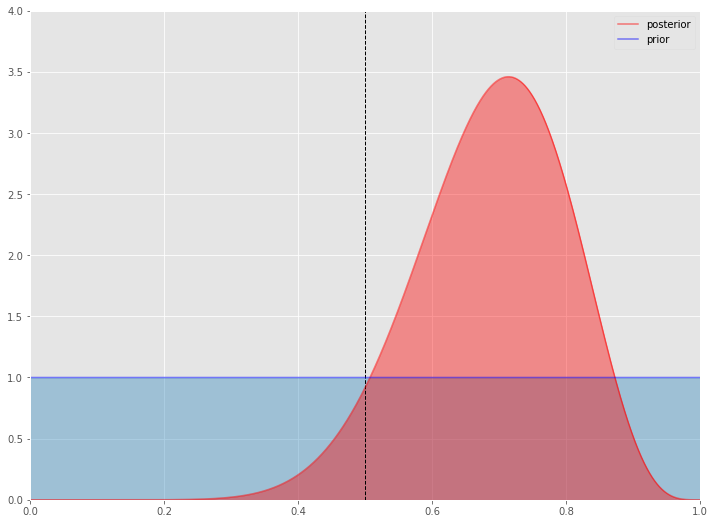
\includegraphics[height=8cm]{coin0.png}
\captionof{figure}{\footnotesize{Prior and posterior distribution in the coin example. The black line corresponds with the well known real value of $p$.}}
\label{coin0}
\end{minipage}
\\$ $ \\
Solving the integral in \eqref{ex} with \eqref{ex1} and \eqref{ex4} we arrive at the final result obtained in the above section
\begin{equation}
P(2heads|D)=\frac{B(13,5)}{B(11,5)}=0.485
\end{equation}
%
%
%
\subsection{Updating the probability distribution for a model} 

As we saw in the coin example, due to the fact that we have not enough data we did not arrive to the real value of $p$. If we would like to be closer to the real one we should continue flipping the coin until the amount of data were enough. If we continue with the coin example and, we say, after throwing 100 times the coin we obtain 56 heads, and then after throwing 500 times the coin we obtain 246 heads,we should obtain a more tiny distribution centered near $p=0.5$ (see fig. \ref{coin1}). In this way, it is clear that in order to confront a parameter model and be more accurate of the most probable (``real") value of it, it is necessary to increase the amount of data (and the capacity for precision) in any experimentation. 
%For example, in the cosmological context, there are a lot of experiments like the ones associated with the barionic acoustic oscilations (BAO), the cosmic microwave background (CMB), the neutrinos background radiation, the redshift survey, etc. (if you are interested in knowing a pedagogical explanation of the different experiments, you can look for \cite{observ}), that can help us to confront our model's parameters (or models) and discriminate them in a more accurately way. 
Then, what we have here is that we will have some model's parameters that has to be confronted with different set of data. There are two ways we can do this: first is regarding the sum of all the sets of data that we have, or consider each data set as the new data, but our prior information has to be set by what we know about the previous information. What is important in bayes statistic is that it doesn't matter wich of the 2 possibilities we choose. In the coin context it means that it is equivalent to start with the prior given in figure \ref{coin1}-a and considering the 500 data we can arrive at the posterior \ref{coin1}-d or start with \ref{coin1}-c as our prior and consider the last 400 data to obtain the same posterior \ref{coin1}-d. \\ $ $ \\
\begin{minipage}{\textwidth}
\centering
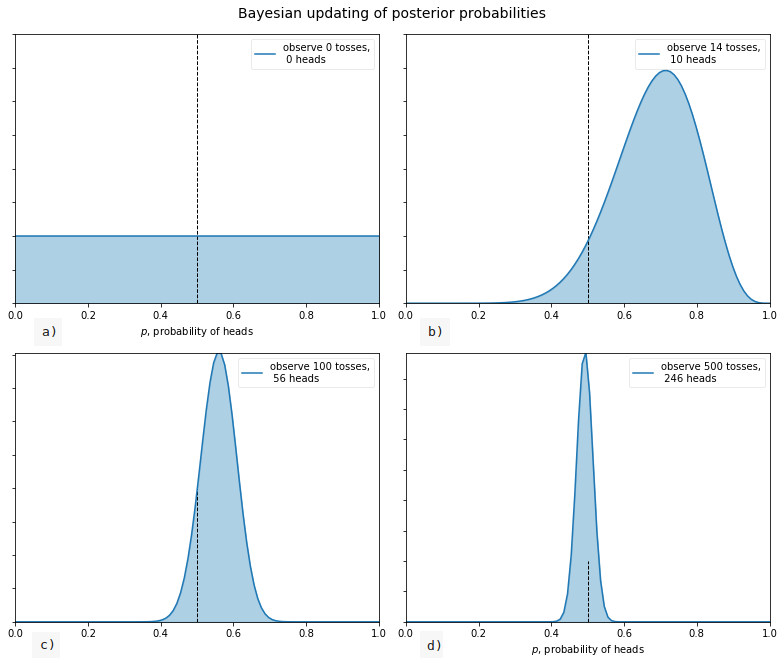
\includegraphics[height=10cm]{coin1.png}
\captionof{figure}{\footnotesize{Posterior distributions of $p$ when our data is increased. Notice that while we continue increasing the experimental results, the posterior distribution starts to be more localized near the real value $p=0.5$.}}
\label{coin1}
\end{minipage}
\\$ $ \\

In fact, if we rewrite Bayes theorem putting explicitly that all probabilities are conditional of some prior information $I$
\begin{equation}\label{BayesTI}
P(\theta,H|DI)=\frac{P(\theta,H|I)P(D|\theta,HI)}{P(D|I)}
\end{equation}
and then we consider a new set of data $D'$, letting the old data become part of the prior information $I'=DI$ we arrive at \cite{AlanH}   
\begin{equation}
P(\theta,H|DI')=\frac{P(\theta,H|I)P(DD'|\theta,HI)}{P(DD'|I)}=P(\theta,H|[DD']I)
\end{equation}
where we can see explicitly the equivalence of the 2 different options for analyzing our results. 
\subsection{About the Likelihood}

We mentioned that the evidence in the Bayes theorem is not usually important when we try to do any inference procedure in the parameter space of a single model. Then, we can fix it as $P(D)=1$ without lost of generality. If we ignore the prior\footnote{It is expected that the real value of a given parameter is independent of the election of the prior.} we can identify the likelihood with $P(H|D)$ and thus by maximizing it we can find the most likely model (or model's parameters) given the data. However having ignored $P(D)$ and the prior this approach cannot give in general a goodness of fit and thus cannot give an absolute probability for a given model. However it can give relative probabilities. In the other side, it is possible to report results independently of the prior by using the \textit{Likelihood ratio}. The likelihood at a particular point in parameter space can be compared with the one that best fit the observations, $L_{max}$. Then we can say that a model is acceptable if the likelihood ratio
\begin{equation}
\Lambda=-2\ln\left[\frac{L(D;\theta,H)}{L_{max}}\right]
\end{equation}
is bigger than a given value.

In the other side, let us assume we have a posterior distribution, which is single-picked. We consider that $\hat \theta$ corresponds with the peak of the distribution (most probable) or the mean
\begin{equation}
\hat \theta =\int d\theta \theta P(\theta,H|D).
\end{equation}
We consider that our model is well-specified and that the expectation value of $\hat \theta$ corresponds with the real value $\theta_0$
\begin{equation}
\langle\hat \theta\rangle=\theta_0,
\end{equation}
then we say that $\hat \theta$ is \textit{unbiased}. Considering a Taylor expansion of the log likelihood
\begin{equation}
\ln L(D;H)=\ln L(D;H_0)+\frac{1}{2}(\theta_\alpha-\theta_{0\alpha})\frac{\partial^2\ln L}{\partial\theta_\alpha \partial\theta_\beta}(\theta_\beta-\theta_{0\beta})+...
\end{equation}
where $H_0$ corresponds with the real model (and/or parameter of the model). In this way we have that the likelihood can be expressed as a multi-variable likelihood given by 
\begin{equation}\label{GLik}
L(D;H)=L(D;H_0)\exp \left[-\frac{1}{2}(\theta_\alpha-\theta_{0\alpha})H_{\alpha\beta}(\theta_\beta-\theta_{0\beta})\right]
\end{equation}
where 
\begin{equation}
H_{\alpha\beta}=\frac{\partial^2\ln L}{\partial\theta_\alpha \partial\theta_\beta}
\end{equation}
is called the \textit{Hessian matrix} and it controls whether the estimates of $\theta_\alpha$ and $\theta_\beta$ are correlated or not. If it is diagonal, the estimates are uncorrelated.

The above expression for the likelihood is a good approximation always that our posterior distribution possess a single-pick. However in a general way the likelihood may not be well described by a gaussian expression at levels wich set the interesting credibility levels. It is worth mentioned that if the data error are Gaussianly distributed, then the likelihood for the data will be a Gaussian function, as well.  In fact, this is always true if the model depends linearly on the parameters \cite{LiV}. In the other side, if the data are not Gaussianly distributed we can resort to the central limit theorem. In this way the central limit theorem will tell us that the resulting distribution will be better approximated by a multi-variate Gaussian \cite{LiV}.
\subsection{Justifying the neglect of the priors}

In this section we are interested in justifying the neglect of the prior in the Bayes theorem. For this, we follow the example given in \cite{RobT}. In this example there are 2 people A and B that are interested on the measurement of a given physical quantity $\theta$. A and B have different prior beliefs regarding the possible value of $\theta$. This discrepancy could be given by the experience, such as the possibility that A and B have made the same measurement in another moment being alone. Let us denote their priors by $P(\theta|I_i)$ $(i=A,B)$ and let us assume that they are described by two Gaussian distributions on mean $\mu_i$ and variance $\Sigma_i^2$. Now, A and B make a measurement together and they obtain the value $\theta_0=m_1$. If we consider that the experiment is such as that our parameters are uncorrelated we can rewrite \eqref{GLik} as
\begin{equation}\label{LikG}
L(D;HI)=L_0\exp\left[-\frac{1}{2}\frac{(\theta-m_1)^2}{\sigma^2}\right]
\end{equation}
Replacing the hypothesis $H$ by the continuous variable $\theta$ the Bayes theorem for the model of A and B is
\begin{equation}
P(\theta|m_1)=\frac{L(m_1;\theta I_i)P(\theta|I_i)}{P(m_1|I_i)}
\end{equation}
where we have used the notation given in \eqref{BayesTI}. Then the posterior of A and B are again Gaussian with means
\begin{equation}
\hat \mu_i = \frac{m_1+(\sigma/\Sigma_i)^2\mu_i}{1+(\sigma/\Sigma)^2}
\end{equation}
and variance 
\begin{equation}
\tau_i^2=\frac{\sigma^2}{1+(\sigma/\Sigma_i)^2}, \ \ (i=A,B)
\end{equation}
Thus if the likelihood is more informative than the prior i.e. $(\sigma/\Sigma)\ll 1$ the posterior means of A and B will converge towards the measured value, $m_1$. As more and more data are obtained one can simply replace the value of $m_1$ in the above equation by the mean $\langle m\rangle$ and $\sigma^2$ by $\sigma^2/N$. Then, we can see that the initial prior $\mu_i$ of A and B will progressively be overridden by the data. This process is ilutrated in figure \ref{gausian1} 
\begin{minipage}{\textwidth}
\centering
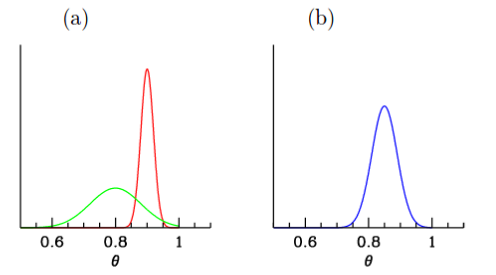
\includegraphics[height=4.5cm]{g1.png}
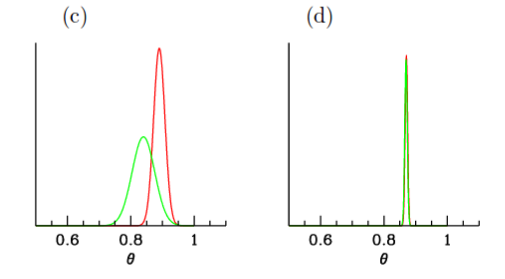
\includegraphics[height=4.5cm]{g2.png}
\captionof{figure}{\footnotesize{Converging views in Bayes inference, taked from \cite{RobT}. A and B have different priors $P(\theta|I_i)$ about a value of $\theta$ (panel (a)). Then, they observe one datum with likelihood $L(\theta;HI)$ (panel (b)), after which their posteriors $P(\theta|m_1)$ (panel (c)) represents their updates. Then, after observing 100 data it can be seen how both posteriors are practically indistinguishable (panel (d))}}
\label{gausian1}
\end{minipage}
\subsection{Chisquare and goodness of fit}

We mentioned that it is necessary to maximize the likelihood in order to obtain the more likely model (or model parameters) given the data. If we consider the Gaussian approximation given in \eqref{LikG} we can see that the likelihood will be maximum always that the quantity
\begin{equation}\label{chi2}
\chi^2\equiv(\theta_\alpha-\theta_{0\alpha})H_{\alpha\beta}(\theta_\beta-\theta_{0\beta})
\end{equation}
is minimum. The quantity $\chi^2$ is usually called \textit{chisquare} and is related with the Gaussian likelihood via $L=L_0e^{-\chi^2/2}$. In this way we can say that the maximizing of a Gaussian likelihood procedure and the minimizing of a chisquare procedure are equivalent. However, as we mentioned before, there are some circumstances where the likelihood can not be well specified by a Gaussian distribution, then, in that cases the chisquare and the likelihood are not longer equivalent. 

We can consider a probability distribution for different values of $\chi^2$ around its minimum. This is the $\chi^2$ distribution for $v=n-M$ degrees of freedom where $n$ is the number of independent data points and $M$ the number of parameters. In this way we can calculate the probability that an observed $\chi^2$ exceeds by chance a value $\hat \chi$ for the correct model. This probability is given by \cite{NR} $Q(v,\hat\chi)=1-\Gamma(v/2,\hat\chi/2)$ where $\Gamma$ is the incomplete Gamma function. Then, the probability that the observed $\chi^2$ (even the correct model) is less that a given value $\hat\chi^2$ is $1-Q$. This statement is strictly true if errors are Gaussian and the model is a linear function of the likelihood, i.e., for Gaussian likelihoods.

If we evaluate the quantity $Q$ in the best fit of the chisquare (i.e. its minimum) we can have a measure of the goodness of the fit. If $Q$ is small (small probability) we can interpret it as:
\begin{itemize}
\item The model is wrong and can be rejected
\item The errors are underestimated 
\item The measurement errors are not Gaussianly distributed.
\end{itemize}
In the other side if $Q$ is too large there are some reasons that could cause such overestimation:
\begin{itemize}
\item Errors have been overestimated
\item Data are correlated or non-independent
\item The distribution is non-Gaussian.
\end{itemize}
\subsection{Contour plots and confidence regions}

Once the best fit parameters are obtained we would like to know if there are confidence regions where other parameters could be consider as a good candidate for our model. The most logical election is to consider parameters inside a compact region around the best fit value. Then, a natural choice is consider regions with a constant $\chi^2$ boundaries. In the case that $\chi^2$ posses more than 1 minimum it is say that we have more than one non-connected confidence region. For multi-variate Gaussian distributions (as the likelihood approximation \eqref{LikG}) these are ellipsoidal regions. In this section we exemplify how to calculate the confidence regions following \cite{LiV}. 

We can consider a little perturbation from the best fit of chisquare $\Delta\chi^2=\chi^2-\chi^2_{best}$. Then we can use the properties of $\chi^2$ distribution to define confidence regions for variations on $\chi^2$ to its minimum. In Table \ref{tableerrors} we can see the typical $68.3 \%$, $95.4\%$ and $99.5\%$ confidence levels as a function of number of parameters for the joint confidence level. In the case of Gaussian distribution (as the likelihood) these correspond to the conventional 1, 2 and 3 $\sigma$.
\begin{table}[h!]
\centering
\begin{tabular}{||l|l|l|l|l||} 
 \hline
$\sigma$ & $p$ & $M=1$ & $M=2$ & $M=3$\\
\hline
$1\sigma$ & $68.3 \%$ & $1.00$ & $2.30$ & $3.53$\\
$2\sigma$ & $95.4 \%$ & $4.00$ & $6.17$ & $8.02$\\
$3\sigma$ & $99.73\%$ & $9.00$ & $11.8$ & $14.20$\\
\hline
\end{tabular}
\caption{\footnotesize{$\Delta \chi^2$ for the conventional $68.3\%$, $95.4\%$ and $99.73\%$ as a function of the number of parameters for the joint confidence level.}}\label{tableerrors}
\end{table}

The general cooking recipe to compute constant-$\chi^2$ confidence regions are as follow: After having found the best fit by minimizing $\chi^2$ (or maximizing the likelihood) and if $Q$ for the best parameters is acceptable, then:
\begin{enumerate}
\item Let $M$ be the number of parameters, $n$ the number of data and $p$ be the confidence limit desired.
\item Solve the equation:
\begin{equation}
Q(n-M,min(\chi^2)+\Delta\chi^2)=p
\end{equation}
\item Find the parameter region where $\chi^2\leq min(\chi^2)+\Delta\chi^2$. This define the confidence region.
\end{enumerate}
\subsection{Marginalization}

It is clear that a model can (in general) depend on more than one parameter. However, most of this parameters $\theta_i$ may be uninteresting. For example, this parameters can  corresponds with nuisance parameters like calibration factors or it may be that we are interested on constraints on only one parameter at the time rather than on the joint constraints on 2 or more parameters simultaneously. Then we marginalize over the uninteresting parameters by
\begin{equation}
P(\theta_1,...,\theta_j,H|D)=\int d\theta_{j+1}...d\theta_{m}P(\theta,H|D)
\end{equation}
where $m$ is the total number of parameters in our model and $\theta_1$,...,$\theta_j$ denote the parameters that we are interested in.

\subsection{Fisher Matrix}

Once we have a set of data it is important to know how accurate we can estimate model parameters. Fisher \cite{Fisher} proposed a way to solve this issue 70 years ago. In this section we review the main results of his work following the procedure given in \cite{LiV}.

First at all we consider again the gaussian likelihood. As we can notice the Heissian matrix $H_{\alpha\beta}$ enclose information of the parameters errors and their covariance. More specifically when all parameters are fixed except one (e.g. the ith parameter) the error on that parameter is $1/\sqrt{H_{ii}}$. These errors are called conditional errors, although they are not usually used.

A quantity that arises naturally with gaussian likelihoods to forecast the precision of a model is the so-called \textit{Fisher information matrix}
\begin{equation}
F_{ij}=-\left\langle \frac{\partial^2 \mathcal{L}}{\partial \theta_\alpha \partial \theta_\beta}\right\rangle
\end{equation}
where 
\begin{equation}
\mathcal{L}=\ln L
\end{equation}
It is clear that $F=\langle H\rangle$. Here average is over observational data. 

As we can see from eq. \eqref{rule4} when we have independent data sets, the complete likelihood is the product of the likelihoods and then the fisher matrix for independent data sets is the sum of the individual fisher matrices. 

A pedagogical and the easiest case is working in the one-parameter case $\theta_i$ and considering a gaussian likelihood. In this scenario we have that
\begin{equation}
\Delta \mathcal{L}=\frac{1}{2}F_{ii}(\theta_i- \theta_{0i})^2
\end{equation}
when $2\Delta\mathcal{L}=1$ and by identifying it with the $\Delta \chi^2$ corresponding to $68\%$ confidence level, we notice that $1/\sqrt{F_{ii}}$ yields the $1-\sigma$ displacement for $\theta_i$. In the general case
\begin{equation}\label{rao}
\sigma_{ij}^2 \geq (F^{-1})_{ij}
\end{equation}
Thus when all parameters are estimated simultaneously from the data the marginalized error is
\begin{equation}
\sigma_{\theta_i}\geq (F^{-1})^{1/2}_{ii}
\end{equation}
The beauty of the Fisher matrix approach is that there is a simple prescription for setting up the Fisher matrix knowing only your model and your measurement uncertainties and that
under the assumption of a gaussian likelihood, the Fisher matrix is the inverse of the covariance matrix. So all you have to do is set up the Fisher matrix and then invert it to obtain the covariance matrix (that is, the uncertainties on your model parameters). In addition if it can be computed quickly, it also enables one to explore different experimental set ups and optimize the experiment.

The whole point of the Fisher matrix formalism is to predict how well the experiment will be able to constrain the model parameters, before doing the experiment and in fact without even simulating the experiment in any detail. We can then forecast the results of different experiments and look at trade offs such as precision versus cost. In other words, we can engage in experimental design.

The $\leq$ in \eqref{rao} is called the Kramer-Rao inequality. We can see that the Fisher information matrix represent a lower bound for the errors. Only when the likelihood is gaussianly distributed the $\leq$ is transformed in $=$. However as we saw in [About the likelihood] a gaussian likelihood is only applicable to some circumstances, being generally impossible to be applied. So the key is to  have a good understanding of our theoretical model in such a way that we can construct a gaussian likelihood.

\subsection{Importance Sampling}

We call importance sampling (IS) to the different techniques of determining properties of a distribution by drawing samples from another one. The basic idea of this procedure is that we consider that the distribution one draws from should be (for a larger number of samples) 
 representative of the distribution of interest, in such case we should infer different quantities of it. In this section we review the basic concepts necessary to understand what IS is following \cite{importancesampling}.

Suppose we are interested in computing the expectation value $\mu_f=E_p[f(X)]$, where $p(x)$ is a probability density of a random variable $X$ and sub-index $p$ means average over the distribution $p$. Then, if now we consider a new probability density $q(x)$ that satisfies $q(x)>0$ whenever $f(x)p(x)\not = 0$, we can rewrite the mean value $\mu_f$ as
\begin{equation}
\mu_f = \int f(x)p(x)dx=\int f(x)\frac{p(x)}{q(x)}q(x)dx=E_q[f(X)w(x)]
\end{equation}
where $w(x)=p(x)/q(x)$ and now we have an average over $q$. In this way if we have a collection of different draws $x^{(1)},...,x^{(m)}$ from $q(x)$, we can estimate $\mu_f$ using this draws as
\begin{equation}
\hat \mu_f = \frac{1}{m}\sum_{j=1}^m w(x^{(j)})f(x^{(j)})
\end{equation}
If $p(x)$ is known only up to a normalizing constant, the above expression can be calculated  as a ratio estimate
\begin{equation}
\hat \mu_f=\frac{\sum_{j=1}^m w(x^{(j)})f(x^{(j)})}{\sum_{j=1}^mw(x^{(j)})}.
\end{equation}
For the strong law of large numbers, in the limit when $m\rightarrow \infty$ we will have that $\hat \mu_f\rightarrow \mu_f$.

In Bayes analysis it can be useful to compute the ratio between evidences for two different models
\begin{equation}\label{importanceratio}
\frac{P'(D)}{P(D)}=E\left[\frac{P'(\theta,D}{P(\theta,D)}\right]_{P(\theta|D)}\simeq \frac{1}{N}\sum_{n=1}^N\frac{P'(D|\theta_n)P'(\theta_n)}{P(D|\theta_n)P(\theta_n)}
\end{equation}
where the samples $\lbrace\theta_n\rbrace$ are drawn from $P(\theta|D)$.

An important result for importance sampling is that if we have a new set of data which is broadly consistent with the current data, in the sense that the posterior only shrinks, we can make use of importance sampling in order to quickly calculate a new posterior including the new data.
\subsection{Combining datasets: Hyperparameter method}

Suppose we are dealing with multiple datasets,  $\lbrace D_1,...,D_N\rbrace$, coming from a collection of different surveys $\left\lbrace S_1,...,S_N\right\rbrace$. Of course we could not be sure, a priori, that all our data surveys are consistent which one another or if there is one or more that are likely to be erroneous. If we were sure that all this datasets are consistent, then it should be enough to update the probability as was seen in [Updating the probability distribution for a model] in order to calculate the new posterior distribution for the parameters that we are interested about. However, because usually we are not sure about this, a way that we can have any information about how much useful is a data survey is by introducing the hyperparameter method. This method was firstly proposed by \cite{hiperp} and \cite{hiperp1} in order to perform a joint estimation of cosmological parameters from combined datasets and it can be used always that we can consider every survey independent between them.

In this section we review the main steps necessary to understand the hyperparameter method following ref. \cite{hiperp1}. If readers are interested in a more explicit explanation of it, they can consult \cite{hiperp} or \cite{hiperp1}.

The basic idea of this process is to introduce a new set of ``hyperparameters" $\alpha$ in our bayesian procedure in order to avoid extra freedom in the parameter estimation process.  This hyperparameters are equivalent to nuisance parameters in such case we need to marginalize over the hyperparameters $\alpha$ in order to recover the posterior distribution, i.e.
\begin{equation}
P(\theta,H|D)=\frac{1}{P(D)}\int P(D|\theta,\alpha,H)P(\theta,\alpha,H)d\alpha
\end{equation}
where we have used the Bayes theorem. Now, it is necessary for the method to assume that the hyperparameters $\alpha$ and the parameters of interest $\theta$ are independent, i.e. $P(\theta,\alpha,H)=P(\alpha)P(\theta,H)$. It is also necessary to assume that each hyperparameter $\alpha_k$ are themselves independent, i.e. $P(\alpha)=P(\alpha_1)P(\alpha_2)...P(\alpha_N)$. In this way we can rewrite the above expression as
\begin{equation}
P(\theta,H|D)=\frac{P(\theta,H)}{P(D|H)}\left[\prod_{k=1}^N\int P(D_k|\theta,\alpha_k,H)P(\alpha_k)d\alpha_k\right]
\end{equation}
Here, the quantity inside square brackets is the marginalized Likelihood over hyperparameters, $L(D;\theta,H)$, and then we can identify the quantity inside the integration as the individual Likelihood, $L(D_k;\theta,\alpha,H)$, for ever $\alpha_k$ and $D_k$; $P(D|H)$ is the evidence and in a typical parameter inference procedure, works as a normalized function, i.e. $P(D|H)=\int P(\theta,H)L(D;\theta,H)$. Notice that by considering $P(a_k)=\delta(\alpha_k-1)$ we relay in the standar approach where no hyperparameters are introduced.  

We add this hyperparameters in order to weight, in a way, every dataset and take away the importance of those data that seem not to be consistent with the other ones. Then, how we can know whether the data support the introduction of hyperparameters? Of course if the datasets are consistent, the introduction of hyperparameters could difficult or give rise to large uncertainties in our estimation. The way that it is possible to response this question is given by the bayesian evidence.

Suppose we have two models, one that considers the introduction of hyperparameters, $H_1$, while the second one is the model without them, $H_0$. The bayesian evidence $P(D|H_i)$ is an important quantity at the moment that we are interested in make a comparison between two different models. In fact, defining the ratio $K$ between two Bayesian evidences
\begin{equation}
K=\frac{P(D|H_1)}{P(D|H_0)}
\end{equation}
we can estimate if it is neccesary to introduce this new parameters to our model, considering the criteria given in the next table:
\begin{table}[h!]
\centering
\begin{tabular}{||l|l||} 
 \hline
 \textbf{K value} & \textbf{Strenght of evidence} \\ [0.5ex] 
 \hline\hline
 $<1$  & Negative (supporting $H_0$)   \\ 
 \hline
 1 to 3 & Weak \\
 \hline 
3 to 10 & Substantial\\
\hline
10 to 30 & Strong\\
\hline
30 to 100 & Very Strong \\
\hline
$>100$ & Decisive\\ [1ex] 
 \hline
\end{tabular}\label{evidence}
\caption{Criteria for the ratio between two Bayesian evidence, taken from \cite{hiperp2}.}
\end{table}

If we consider a Gaussian Likelihood and we consider a maximum entropy prior assuming that on average the hyperparameters weight are unity, we can rewritte the marginalized Likelihood function $L(D;\theta,H_1)$ for model $H_1$ as
\begin{equation}
P(D;\theta,H_1)=\prod_{k=1}^N\frac{2\Gamma(\frac{n_k}{2}+1)}{\pi^{n_k/2}|V_k|^{1/2}}(\chi_k^2+2)^{-\left(\frac{n_k}{2}+1\right)}
\end{equation}
obtaining an explicitly functional form for $K$ given by
\begin{equation}
K=\prod_{k=1}^N\frac{2^{n_k/2+1}\Gamma(n_k/2+1)}{\chi^2_k+2}e^{-\chi_k^2/2}.
\end{equation}
Here $\chi_k$ is the one given by \ref{chi2} for every dataset and $n_k$ is the number of points content on $D_k$. Notice that if we have a set of independent samples for $H_0$, we can compute an estimate for $K$ with the help of equation \eqref{importanceratio}. 
%\subsubsection{Computing Fisher matrices}


%\subsection{Summary}

%In order to make a Bayesian parameter inference we showed that the most important artifact necessary to know is the Bayes theorem. This theorem depend basically of 4 components: the prior, the likelihood, the posterior and the evidence. If we are only interested in the parameter inference procedure for a single model, we saw that we can ignore the posterior and the prior, being only the likelihood important for calculating the posterior (the posterior probability distribution for our parameter). Then, we can consider the most probable value for our parameter the one associated with the maximum value of our likelihood.
%
%In the other side we saw that there are some circumstances in which we can rewrite  

\section{Numerical tools}

In a typical scenario it is not possible to compute the posterior analytically in our Bayesian inference procedure. In this way it is important to know, once we have all the necessary mathematical tools to make a bayesian estimation, all the numerical tools at our disposal that can help us in our parameter estimation. Of course we could have several numerical candidates that could help us in this homework, but in this section we present only the typical one (and the easier) used in cosmology: the Monte Carlo Markov Chain (MCMC) with the Metropolis Hasting algorithm (MHA). Additionally in this section we present some useful details that we have to take into account if we want to make efficient our computation. 

\subsection{MCMC techniques for parameter inference}

The purpose of a Monte Carlo Markov Chain (MCMC) algorithm is to construct a sequence of points in a parameter space (called ``chain") in order to evaluate the posterior of eq. \eqref{BayesT} for the usual case where analytical solutions do not exist or are insufficiently accurate. In this section we review the basics results for this procedure in a simplistic way but for curious readers it is recommendable to see \cite{mcmc1},\cite{mcmc2}, \cite{mcmc3} or only for markov chains \cite{mcmc4}.

A sequence $X_1,X_2,...$ of random elements of some set is a \textit{Markov chain} if the conditional distribution of $X_{n+1}$ given $X_1,...,X_n$ depends on $X_n$ only. In other words a Markov chain is a process where we can do predictions of the future based only in the information given at the present. An important property of a Markov chain is that they can be shown to converge to a stationary state were successive elements of the chain are samples from the target distribution, in our case the posterior $P(\theta,H|D)$. In this way we can estimate all the usual quantities of interest from it (mean, variance, etc). The number of points required to get good estimates is said to scale linearly with the number of parameters, so very quickly become much faster than grids as the dimensionality increases.

The target density is approximated by a set of delta function
\begin{equation}
p(\theta,H|D)\simeq \frac{1}{N}\sum_{i=1}^N \delta(\theta-\theta_i)
\end{equation}

Then, the posterior mean is calculated as
\begin{equation}
\langle\theta\rangle=\int d\theta \theta P(\theta,H|D)\simeq \frac{1}{N}\sum_{i=1}^N\theta_i
\end{equation}
where $\simeq$ follows because the sample $\theta_i$ are generated from the posterior by construction. Then, we can estimate any integrals (such as the mean, variance, etc) as
\begin{equation}
\langle f(\theta)\rangle \simeq\frac{1}{N}\sum_{i=1}^N f(\theta_i)
\end{equation}

As was mentioned, in a Markov chain it is necessary to generate a new point $\theta_{i+1}$ in our chain from the present point $\theta_i$. However, as it is expected, we need a criteria for accepting (or refusing) this new point depending if it results to be better for our model or not. In the other side, if this new step is better than the previous one, we would like not always accept it, since it could be the case that we were converging to a local maximum in our parameter space and therefore not completely mapping it. The simplest algorithm that contains all this information in its methodology is known as the Metropolis-Hasting algorithm and in what follows we explain in what it consists.
\subsubsection{Metropolis Hasting algorithm}

In the \textit{Metropolis Hasting algorithm} (MHA) \cite{metr} it is neccesary to start from a random initial point $\theta_0$, with associated posterior probability $p_0=p(\theta_0,H|D)$. We need to propose a candidate $\theta_c$ by drawing from the \textit{proposal distribution} $q(\theta_0,\theta_c)$. Then, the probability of acceptance of a new point is given by
\begin{equation}
p(acceptance)=min\left[1,\frac{p_cq(\theta_c,\theta_0)}{p_0q(\theta_0,\theta_c)}\right]
\end{equation}
If the proposal distribution is symmetric, the algorithm is reduced to the \textit{Metropolis algorithm}
  \begin{equation}
  p(acceptance)=min\left[1,\frac{p_c}{p_0}\right]
  \end{equation}
In this way the complete algorithm can be expressed following this steps:
\begin{enumerate}
\item Choose a random initial condition $\theta_0$ in parameter space and compute the posterior distribution
\item Generate a new candidate from a proposal distribution in the parameter space and compute the corresponding posterior distribution
\item Accept (or not) the new point with the help of the Metropolis Hasting algorithm
\item If the point is not accepted, repeat the previous point in the chain
\item Repeat step 2-4 until you have a chain large enough
\end{enumerate}

\subsubsection{A first example in parameter inference using a MCMC technique with a MHA}

In order to exemplify the numerical tools learned in this section, let us 
go back to the example of the coins seen in subsection [Bayes theorem, prior and posterior distributions]. Because we are interested that the reader understands what is the basic procedure given in this section, let us only try to estimate what is the value of $p$ (or region of values for $p$) that best matches our data (the 14 times that the coin was trough). For it we calculate the posterior distribution \eqref{ex4} using the MHA. 

As before we consider a Likelihood given by a binomial distribution \eqref{ex2} and a normal distributed prior \eqref{ex3} ($a=b=1$). As our first ``guest" for $p$ we take $p_0=0.1$. We generate a new candidate $p_c$ as $p_c=p_i+G(p_i,\sigma)$, where $G(p_i,\sigma)$ is our Gaussian proposal distribution centered at $p_i$ and variance $\sigma=0.1$; $p_i$ is the current value of $p$ that for our first step is $p_i=p_0$. Then, we compute the Metropolis Hasting algorithm in a Python code as can be seen in appendix [A]. Our final result,  fig. \ref{posteriord}, was a posterior distribution that matches very well with the posterior that was calculated analytically. Notice that we have plotted our $95\%$ confidence regions (black line). 

%\begin{figure}[h!]
\begin{minipage}{\textwidth}
\centering

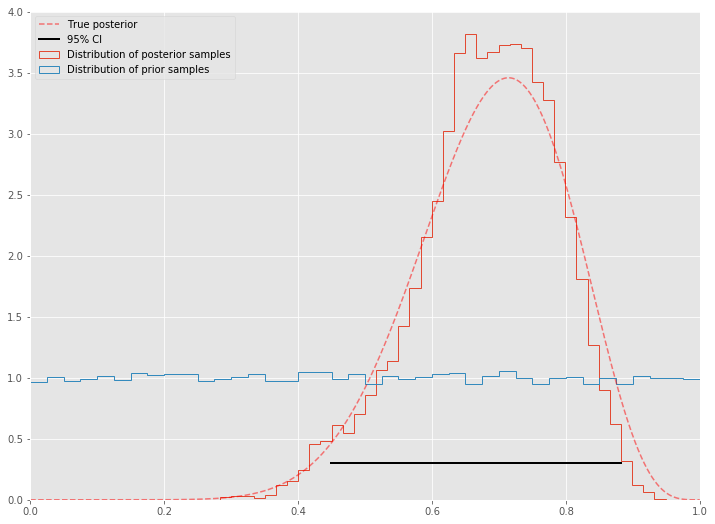
\includegraphics[height=7cm]{posterior.png}
\captionof{figure}{\footnotesize{Posterior distribution for our example. We plot the prior distribution (blue), true posterior (dashed-red) and the posterior calculated by the MHA (red). We plot $95\%$ confidence region for the estimation of $p$.}}
\label{posteriord}
\end{minipage}\\
%\end{figure}

To complete the example we show in figure \ref{chain1} the Markov Chain generated by our code. We can notice that the chain oscillates around a middle value. This behavior is expected due to the fact that we have not enough data to constrain more accurately the value of $p$ and then there are several values for $p$ that can matches with enough precision our data.   

\begin{minipage}{\textwidth}
\centering
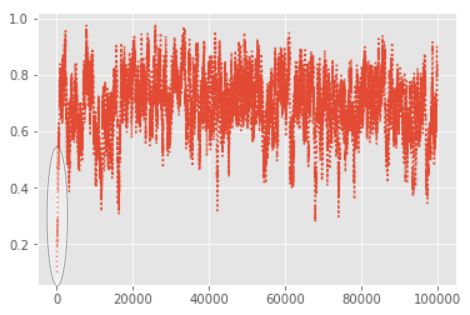
\includegraphics[height=6cm]{chain1.png}
\captionof{figure}{\footnotesize{Markvov chain. We use $p_0=0.1$ as our first ``guest" for $p$. }}
\label{chain1}
\end{minipage}\\ $ $ \\

Note: In appendix [A] we computed our MCMC algorithm using an explicit code of the MCMC process. However, in Python there are some modules that can help us to simplify our life. For example PyMC is a Python module that implements statistical models and fitting algorithms, including the MCMC algorithm. We use this module at the end of this section . Wapplying the tools learned to a complete work session.

\subsubsection{Convergence test} 
It is clear that we need a test to know when our chain has converged. However we need to be warned that the point in our chain is not in a "false convergent point" or a locally maximum point. In this way we need that our rule takes into account this possible difficulty. The simplest way (the informal way) to know if our chain is converging is running several chains starting with different proposal initial point for the parameter that we are interested about to estimate. Then, if we see, by eye, that all the chains looks to converge to a single region of the possible value for our parameter, we could consider that our chains are converging to that region. 

 Taking again the experiment of the coins, we can run several chains for the above example and try to estimate if the value (the region) of $p$ that we found is an sttionary value (region). In figure \ref{chain2} we plotted 5 different Markov chains with initial ``guest" condition $p=0.2,0.3,0.5,0.7,0.9$. As we expected from the analytical result, all the chains looks to concentrate near the same value.

\begin{minipage}{\textwidth}
\centering
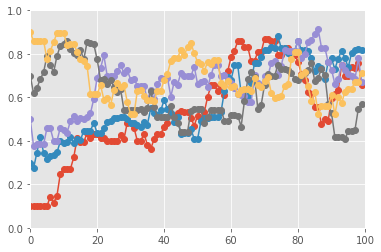
\includegraphics[height=6cm]{chain22.png}
\captionof{figure}{\footnotesize{Multiple MCMC. We calculate 5 Markov chains to estimate convergence of our chains.}}
\label{chain2}
\end{minipage}


The above convergence method explained is very informal and we would like to have a better way to ensure that our result is correct. The classical test used for it is the \textit{Gelman-Rubin} (1992) convergence criterion. This is (following \cite{LicV2}, \cite{AlanH}) by starting $M$ chains with very different initial point and $N$ points per chain. Then if $\theta_i^j$ is a point in parameter space of position $i$ and chain $j$, we need to compute the mean of each chain 
\begin{equation}
\langle\theta^j\rangle =\frac{1}{N}\sum_{i=1}^N \theta_i^j
\end{equation}
and the mean of all the chains
\begin{equation}
\langle\theta\rangle =\frac{1}{NM}\sum_{i=1}^N\sum_{j=1}^M\theta_i^j.
\end{equation}
Then the chain-to-chain variance $B$ is
\begin{equation}
B=\frac{1}{M-1}\sum_{j=1}^M(\langle\theta^j\rangle-\langle\theta\rangle)^2
\end{equation}
and the average variance of each chain is
\begin{equation}
W=\frac{1}{M(N-1)}\sum_{i=1}^N\sum_{j=1}^M(\theta_i^j-\langle\theta^j\rangle)^2
\end{equation}
If our chains converge, $W$ and $B/N$ must agree. In fact we say that the chain converges when the quantity
\begin{equation}
\hat R=\frac{\frac{N-1}{N}W+B(1+\frac{1}{M})}{W},
\end{equation}
which is the ratio of the two estimates, approach to unity. A typical convergence criteria is when $\hat R<1.03$. 

\subsubsection{Some useful details}

\textit{About the proposal distribution.} The choice of a proposal distribution $q$ is crucial for the efficient exploration of the posterior. In our example we used a Gaussian-like distribution with a variance (step) $\sigma=0.1$. This value was taken because we explored, by hand, different values for $\sigma$ and we took the one that looked to approach more quickly to the real main value of $p$. If the scale of $q$ is too small compared with the scale of the target in the sense that the typical jump is small, then the chain may take a very long time to explore the target distribution (left side of the plot) which imply that the algorithm will be very inefficient. As we can see in figure \ref{chainprop} (left side), considering a prior for $p=0.8$, the number of points that we plot is not enough for the system move to its real posterior distribution. In the other side, if the scale of $q$ is too large, the chain gets stuck and it does not jump very frequently (right side of the figure) which implies that we will have different "picks" in our posterior distribution.    

\begin{minipage}{\textwidth}
\centering
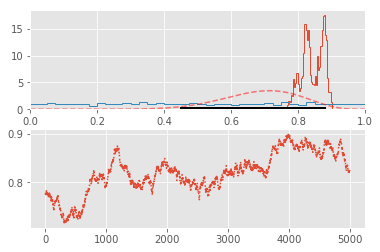
\includegraphics[height=5.5cm]{chain2.png}
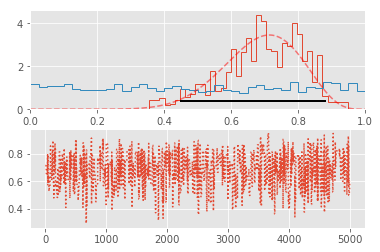
\includegraphics[height=5.5cm]{chain3.png}
\captionof{figure}{\footnotesize{Two Markov chains considering different variance for our Gaussian proposal distribution. Left side correspond with taking $\sigma=0.003$, while right side correspond with $\sigma = 0.8$.}}
\label{chainprop}
\end{minipage}\\ $ $ \\

In order to fix this issue in a more efficient way, it is recommendable to run an exploratory MCMC, compute the covariance matrix from the samples, and then re-run with this covariant matrix as the covariance of a multivariate Gaussian proposal distribution. Of course, this process can be computed a couple of times before to run the ``real" MCMC.\\

\textit{About the burn-in.} It is important to notice that when we start a chain we will have a region of points outside the stationary region where the chain converge (In our chain we could consider those points as the ones inside the ellipse in figure \ref{chain1}). This early part of the chain (called ``burn-in") must be ignored and then the dependence on the starting point must be lost. For it, it is important to have a convergence test which can help us to know when the chain has converged.\\

 \textit{Thinning the chains}.- There are several bayesian statisticians that usually thin its MCMC, it is, they do not prefer to save every step given by the MCMC; instead, they prefer to save a new step each time $n$ steps have taken place. An obvious consequence that follows by thinning the chains is that the amount of autocorrelation is reduced. However, as long as the chains are thinned, the precision for the estimated parameters is reduced \cite{thin}. Thinning the chains can be useful in other kind of circumstances, for example, if we have limitations in memory. Notice that thinning a chain does not yield incorrect results; it yields correct results but less efficient than using the full chains.       
\\

\textit{Autocorrelation proves}.- A complementary way to look for convergence in a MCMC estimation is by looking for the autocorrelation between the samples. The $lag\ k$ autocorrelation is defined as the correlation between every sample and the sample $k$ steps before. It can be quantified as \cite{autocor}
\begin{equation}
\rho_k=\frac{Cov(X_t,X_{t+k})}{\sqrt{Var(X_t)Var(X_{t+k})}}=\frac{E[(X_t-X)(X_{t+k}-X)]}{\sqrt{E[(X_t-X)^2]E[(X_{t+k}-X)^2]}}
\end{equation}
where $X_i$ is the i-th sample and $X$ is the mean of the samples. This autocorrelation should become smaller as long as $k$ increases (this means that samples start to become independent).\\

\textit{Metropolis Coupled Markov Chain Monte Carlo ($MC^3$)}\textcolor{red}{(No estoy seguro si dejarlo o no)}.- It is easy to see that it could be a little problematic if our Likelihoods possesses local maxima. The $MC^3$ is a modification of the standard MCMC algorithm that consist in running several Markov Chains in parallel to explore the target distribution for different  ``temperatures", and then simplify the way we sample our parameter space and help us to avoid this local maxima. In this little section we exemplify the basic idea of this algorithm following \cite{mcmcmc}. If you are interested in a more extensive explanation of this algorithm, or a modification to make dynamical the temperature of the chains, please consult reference \cite{mcmcmc}.

We consider a tempering version of the posterior distribution $P(\theta,H,T|D)$
\begin{equation}
P(\theta,H,T|D) \propto L(\vec\theta,D)^{1/T}P(\theta,H)
\end{equation}
where $L$ is the Likelihood and $P(\theta,H)$ the prior. Notice that for higher $T$, individual peaks of $L$ becomes flatter, making the distribution easier to sample with a MCMC algorithm. Now, we have to run N chains with different temperatures assigned in a ladder $T_1<T_2<...<T_N$, usually taken with a geometrically distributed division, with $T_1=1$. The coldest chain $T_1$ is the one that sample the posterior distribution more accurately and behaves as a typical MCMC. Then, we define this chain as the main chain. The other chains are running in such a way that they can cross local maximum Likelihoods easier and transport this information to our main chain.  

The chains independently explore the landscape for certain number of generations. Then, in a pre-determined interval the chains are allowed to ``swap" its actual position with a probability
\begin{equation}
A_{i,j}=min\left\lbrace\left(\frac{L(\theta_i)}{L(\theta_j)}\right)^{1/T_j-1/T_i},1\right\rbrace .
\end{equation}
In this way, if a swap is accepted, chains $i$ and $j$ must exchange its current position between them in parameter space, then chain $i$ have to be on position $\theta_j$ and chain $j$ have to move to position $\theta_i$. 

We can see that, since the hottest chain $T_{max}$ can access easier to all the modes of $P(\theta,H,T_{max}|D)$, then it can propagate its position to colder chains, to be precises it can propagate its position to the coldest chain $T=1$. At the same time, the position of colder chains can be propagated to hotter chains, allowing them to explore the entire prior volume.   
\\

\textit{\textcolor{blue}{(Monte Carlo Sequential Importance Sampling (MCSIS) `?ser\'ia bueno agregarlo?)}}
\\ $ $

\textit{More samples.-}The generation of the elements in a Markov chain is probabilistic by construction and it depends on the algorithm that we are working with. The MHA is the easiest algorithm used in bayesian inference. However there are several other algorithms that can help us to fulfill our mission. For instance, some of the most popular and effective ones apart of the MHA are the Gibbs sampling (GB) (see e.g. \cite{gibbs1,gibbs2}), the Hamiltoninan Monte Carlo (see e.g. \cite{hamiltonian1,Hamiltonian2}) or the Adaptative Metropolis Hasting AMH (see e.g. \cite{importance}).\\
 
 \subsection{A first complete session work: Adjusting a straight-line}

In this section we apply all that we have learned until now to the simplest example: adjusting a stright-line. This is, we assume that we have a certain theory where our meassurements should be in a stright line. Then, in order to apply our technics, we simulate several datasets along a given line. In the other side, one of the principal topics that we want to analize is the hyperparameter method and how it works. In this way, we apply our analysis for two different examples. First, we consider that we have 2 datasets took from the same stright-line but with different errors, while in the second case we consider that we have two datasets but now we simulate bout of them from different stright-lines and different errors. In our analysis we used the PyMC3 module [red] implemented in Python. Our complete code can be seen in ref. [ref]. This code is so simple to use and can be modified very easily if a new model should be tested. I recommend you to use the archive called ``new model" where you will find a blanck proyect where you can give to it your data and your model and by running all the notebook, you can obtain all the analysis that we will see in this section. You will find too in the same archive several notes that could help you to programing your model with PyMC3. 

\subsubsection{Case 1}

In this example we start by considering that our measurements for a given theory where a straight-line, $y=a+bx$, is the one that it is expected is given by the data shown in figure \ref{data_1}. We call this case as \textit{Case 1}. This two datasets, D1 and D2, were generated from the line $y=3+2x$ adding a gaussian error to each data in our datasets. For D1 we add an error with a standard desviation $\sigma_1 = 0.3$, while for D2 we add $\sigma_2 = 0.2$. Then, what we would like to estimate are the parameters of the model, i. e. $a$ and $b$. In what follows we will analyze this data with and without the hyperparameter method and discuss in detail our results.

\begin{minipage}{\textwidth}
\centering
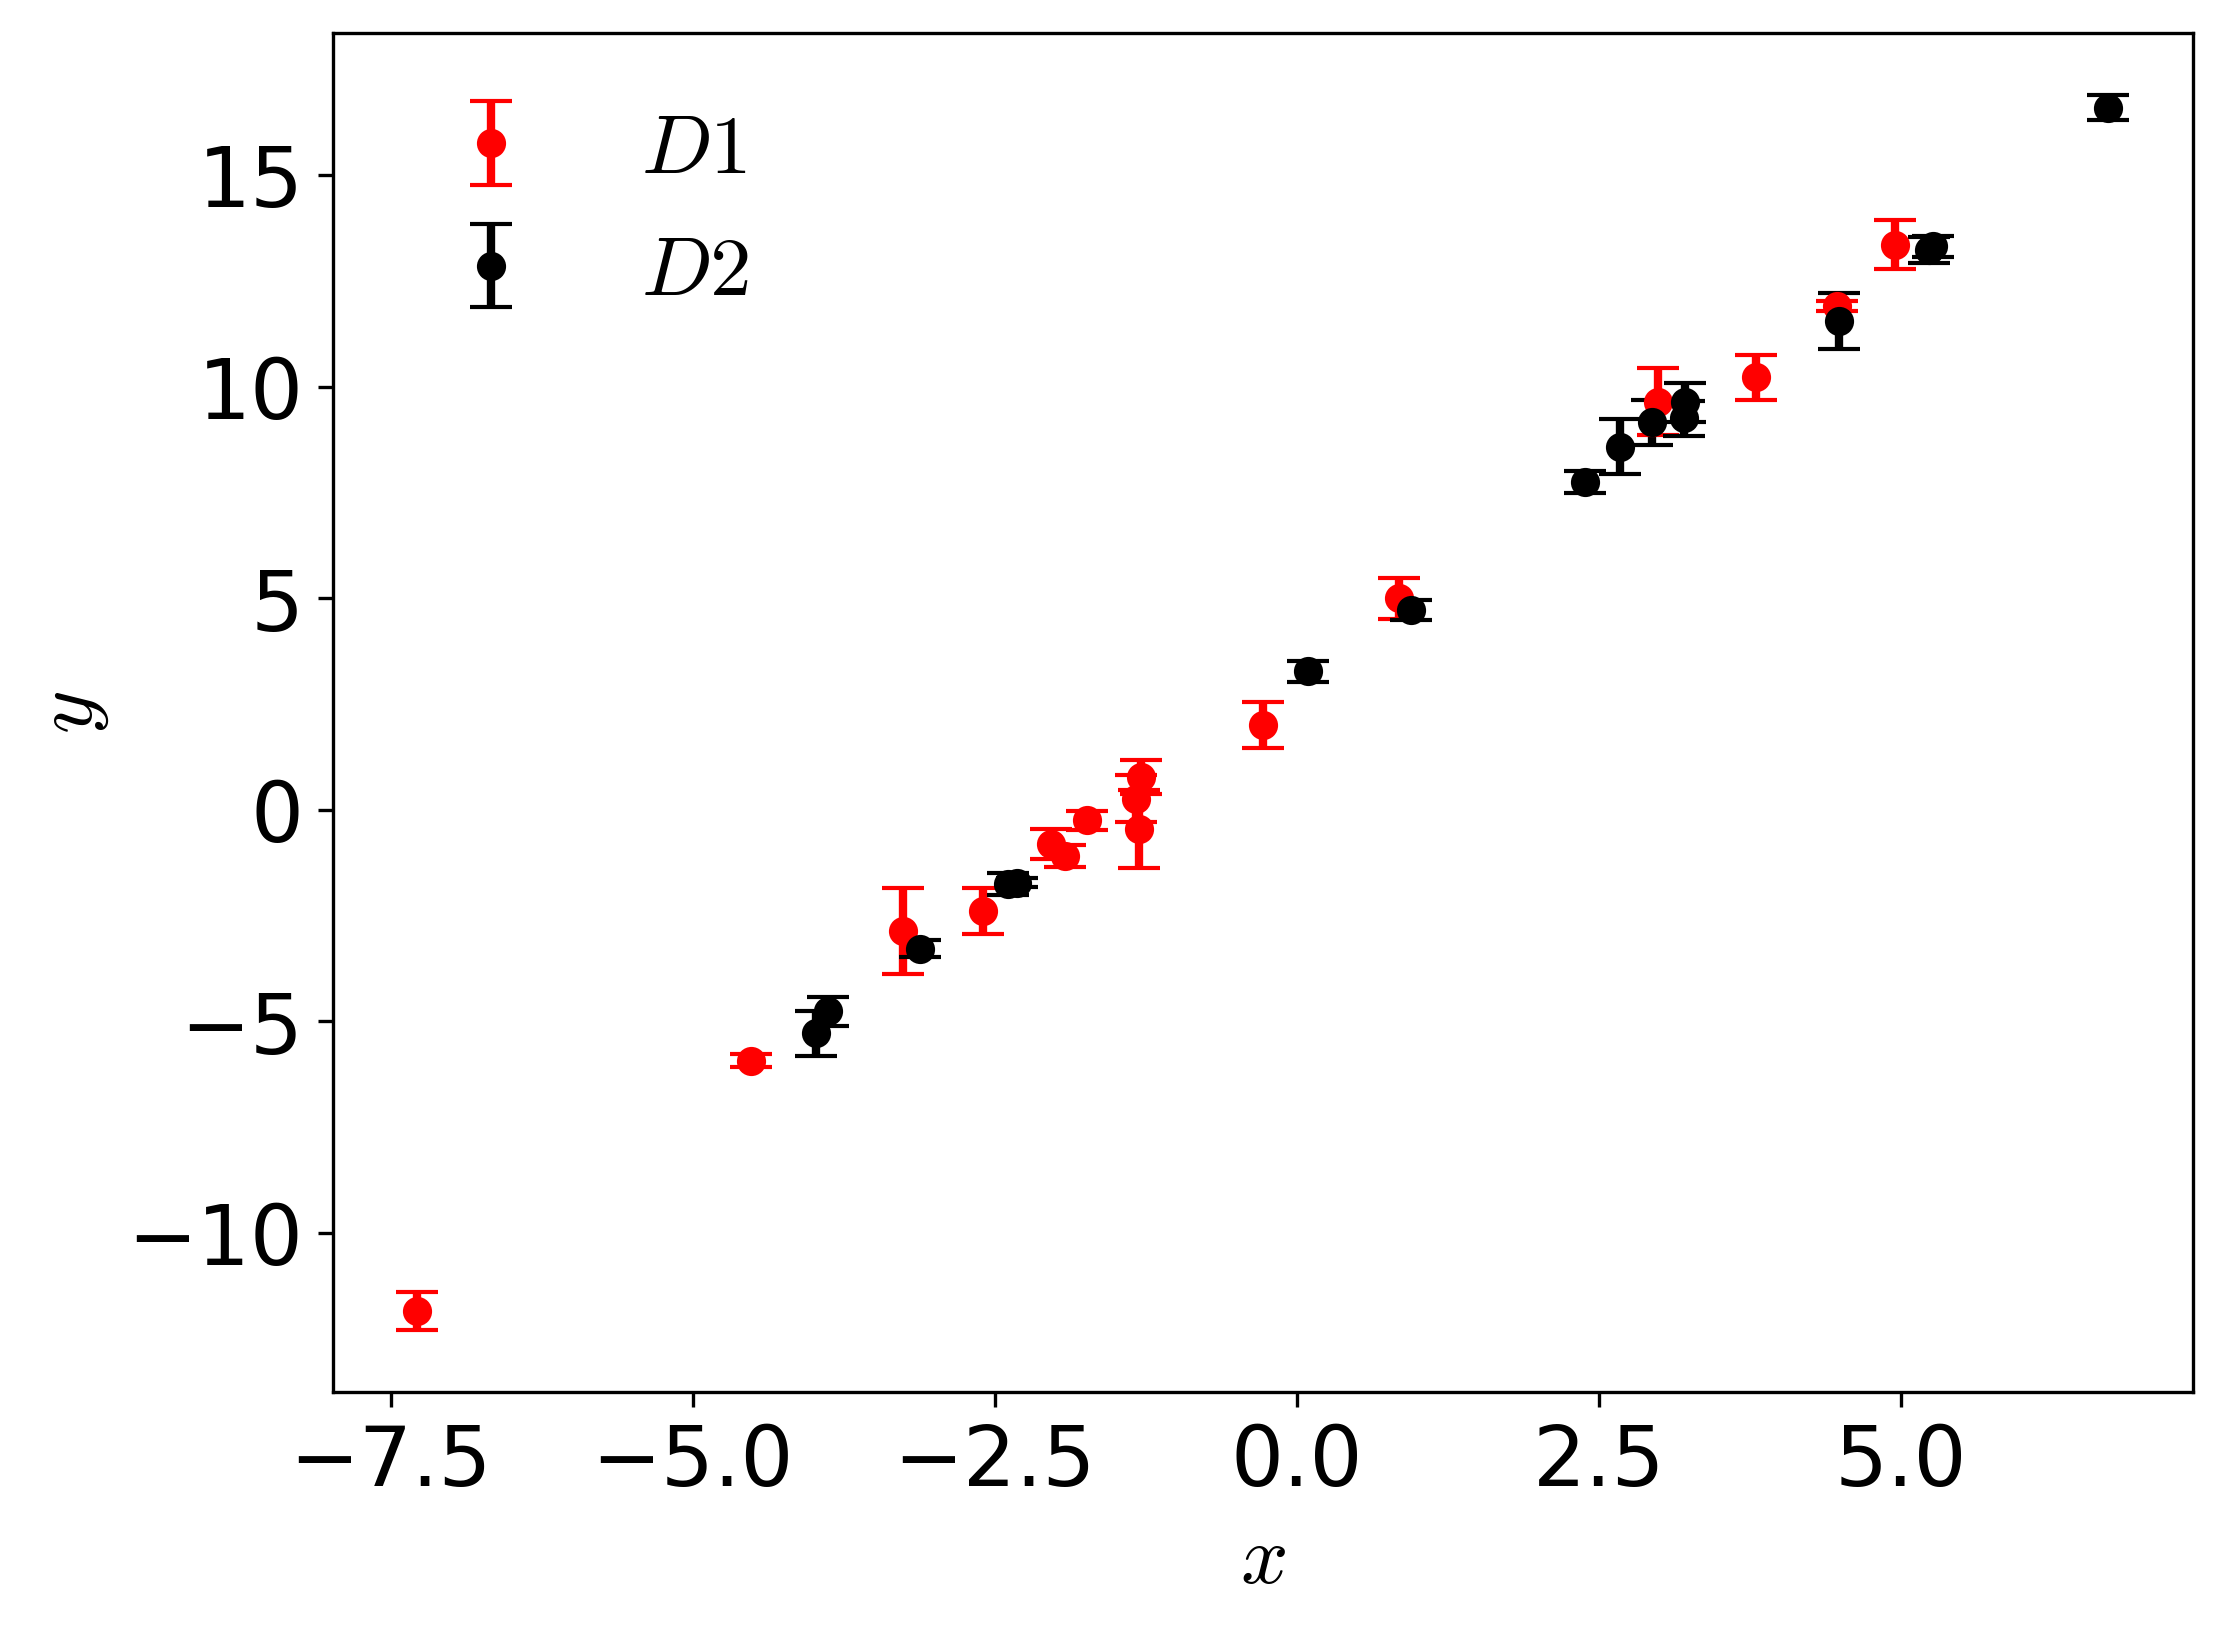
\includegraphics[height=8cm]{data_1.png}
\captionof{figure}{\footnotesize{Datasets $D_1$ and $D_2$ meassured by our stright-line theory.}}
\label{data_1}
\end{minipage}

\textit{Case without hyperparameters. Model $H_0$.-} Before to make a Bayesian estimation it is necessary to specify our priors. As we have seen a good prior is a non informative one. Suppose we only know the boundary limits for $a$ and $b$ (we can see them by eye in our data). Then we consider the flat priors
\begin{equation}
a \propto U[0,5] \ \ \ \text{and} \ \ \ b \propto U[0,3]
\end{equation}
where $U[\alpha,\beta]$ are uniform distributions with lower limit $\alpha$ and upper limit $\beta$.

If now we consider that there are values for $a$ and $b$ for which our data matches better, then from [eq] we can write our likelihood as
\begin{equation}
L(D;recta)\propto \exp\left[-\sum_d \frac{(y_d-y)^2}{2\sigma_d^2}\right]
\end{equation}
where $y_d$ are our data taked from the dataset $D=D_1+D_2$ and $\sigma_d$ its errors.

Now we can generate our MCMC with the MHA. In our analysis we ran 6 chains with 10,000 steps for each one. We ran each chain with a temperature $T=2$ and we thinned them each 50 steps. We can see our results in table \ref{tabla1} and figure \ref{chain}. Notice that there are some regions where the frequency of events in our sample are increased. So we can say that such parameter regions looks to be more likely to match with the data. Additionally we compute the Gelman-Rubin criterion for each variable in order to verify that our results converged. We can see from table \ref{tabla1} that this number is very similar to 1 in such case  implies that our convergence criterion is fulfill.

\begin{table}[h!]
\centering
\begin{tabular}{||l|l|l|l||} 
 \hline
 & \textbf{Promedio} & \textbf{Desv. Est.} & \textbf{Gelman-Rubin} \\ [0.5ex] 
 \hline\hline
$a$ & 2.982407 & 0.047978 & 1.000200 \\
\hline
$b$ & 1.994251 & 0.013490 & 1.000352\\ [1ex] 
 \hline
\end{tabular}
\caption{\footnotesize{Our means obtained in our Bayesian estimation for model $H_0$. We also calculated the Gelman-Rubin criterion for each parameter.}}
\label{tabla1}
\end{table}

\begin{minipage}{\textwidth}
\centering
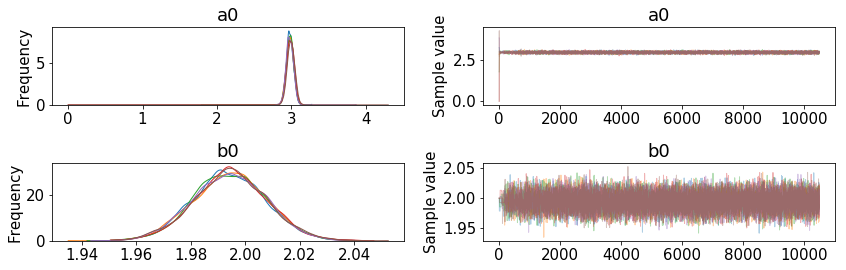
\includegraphics[height=5cm]{chain_new.png}
\captionof{figure}{\footnotesize{Results of our sample in our Markov chains for model $H_0$.}}
\label{chain}
\end{minipage}

Now we need to continue with the autocorrelation plots. As we mentioned, we need that this plots been small as long as k increases in order to consider that our analysis is converging. We can see in figure \ref{autocorr} such plots and notice that our convergence criteria is fulfill.

\begin{minipage}{\textwidth}
\centering
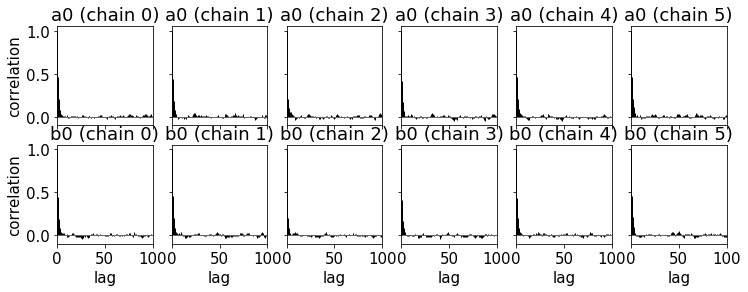
\includegraphics[height=5cm]{autocorr_1.png}
\captionof{figure}{\footnotesize{Autocorrelation plots for model $H_0$.}}
\label{autocorr}
\end{minipage}
\\$ $

Finally in figure \ref{contour_1} we show the typical $1-4\ \sigma$ confidence regions. We also plot in red the real value for our parameters. As we can notice the real value for $a$ and $b$ are inside 1 standard deviation of our estimations by our inferential method. Then, in this Case 1 we can see that the model $H_0$ looks to be a very good estimation procedure.

\begin{minipage}{\textwidth}
\centering
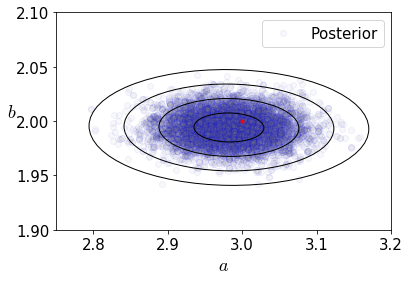
\includegraphics[height=5cm]{contour_1.png}
\captionof{figure}{\footnotesize{Confidence regions for our parameters for model $H_0$.}}
\label{contour_1}
\end{minipage}\\ $ $

\textit{Case with hyperparameters. Model $H_1$.-} Now it is time to prove our h. Model $H_1$yperparameter method. In this case our Likelihood can be written from [ref] as
\begin{equation}
L(D;\theta,H_1)=\prod_{k=1}^N\frac{2\Gamma(\frac{n_k}{2}+1)}{\pi^{n_k/2}|V_k|^{1/2}}\left[\frac{(y_d-y)^2}{2\sigma_k^2}+2\right]^{-\left(\frac{n_k}{2}+1\right)}
\end{equation}

Now, similar than in the last procedure we compute the posterior with our flat priors and using 6 chains with 10,000 steps for each one. Our results and autocorrelation plots can be seen in table \ref{tab} and figure \ref{autocorr_2}. Comparing tables \ref{tabla1} and \ref{tab} we can notice that bout procedures looks to be very similar. In fact, we can notice that the confidence regions for bout approximations, fig. \ref{contour_1} and \ref{contour_2}, are similar as well. So, what method is better? By eye we could say that the method with hyperparameters is as good as the one without them, but what we need to compute in order to be sure of it is the ratio $K$ between bout models. We obtained from [eq] 
\begin{equation}
K = 3
\end{equation}
Then, comparing with table [ref] we can say that the evidence for $H_1$ to be better that $H_0$ is weak, in such case should be better to work with $H_0$ as we explained before.

\begin{table}[h!]
\centering
\begin{tabular}{||l|l|l|l||} 
 \hline
 & \textbf{Promedio} & \textbf{Desv. Est.} & \textbf{Gelman-Rubin} \\ [0.5ex] 
 \hline\hline
$a$ & 2.974059 	 & 0.038583 & 1.000229 \\
\hline
$b$ & 1.995189 & 0.010611 	 & 1.000044\\ [1ex] 
 \hline
\end{tabular}
\caption{\footnotesize{Our means obtained in our Bayesian estimation for model $H_1$. We also calculated the Gelman-Rubin criterion for each parameter.}}
\label{tab}
\end{table}

\begin{minipage}{\textwidth}
\centering
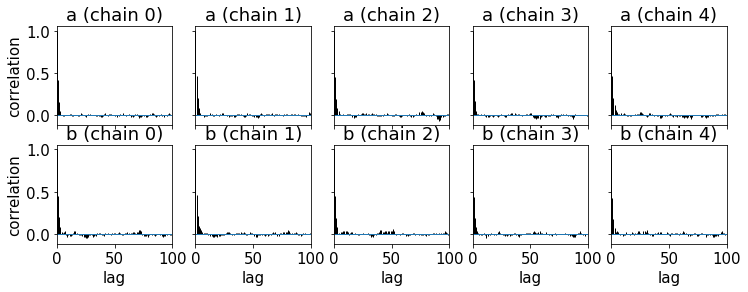
\includegraphics[height=5cm]{autocorr_2.png}
\captionof{figure}{\footnotesize{Autocorrelation plots for model $H_1$.}}
\label{autocorr_2}
\end{minipage}
\\$ $

\begin{minipage}{\textwidth}
\centering
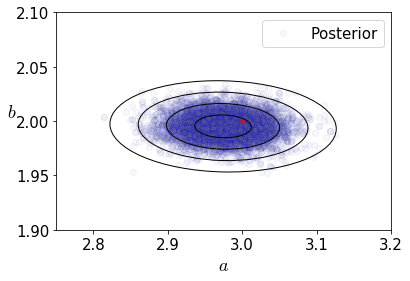
\includegraphics[height=5cm]{contour_2.png}
\captionof{figure}{\footnotesize{Confidence regions for our parameters for model $H_1$.}}
\label{contour_2}
\end{minipage}\\ $ $

Finally, in order to exemplify our results, let us plot in figure \ref{stright1} our data with the stright-line inferred by the mean parameters of bout models. As we expected our estimation fit so well  to our data for bout cases.  

\begin{minipage}{\textwidth}
\centering
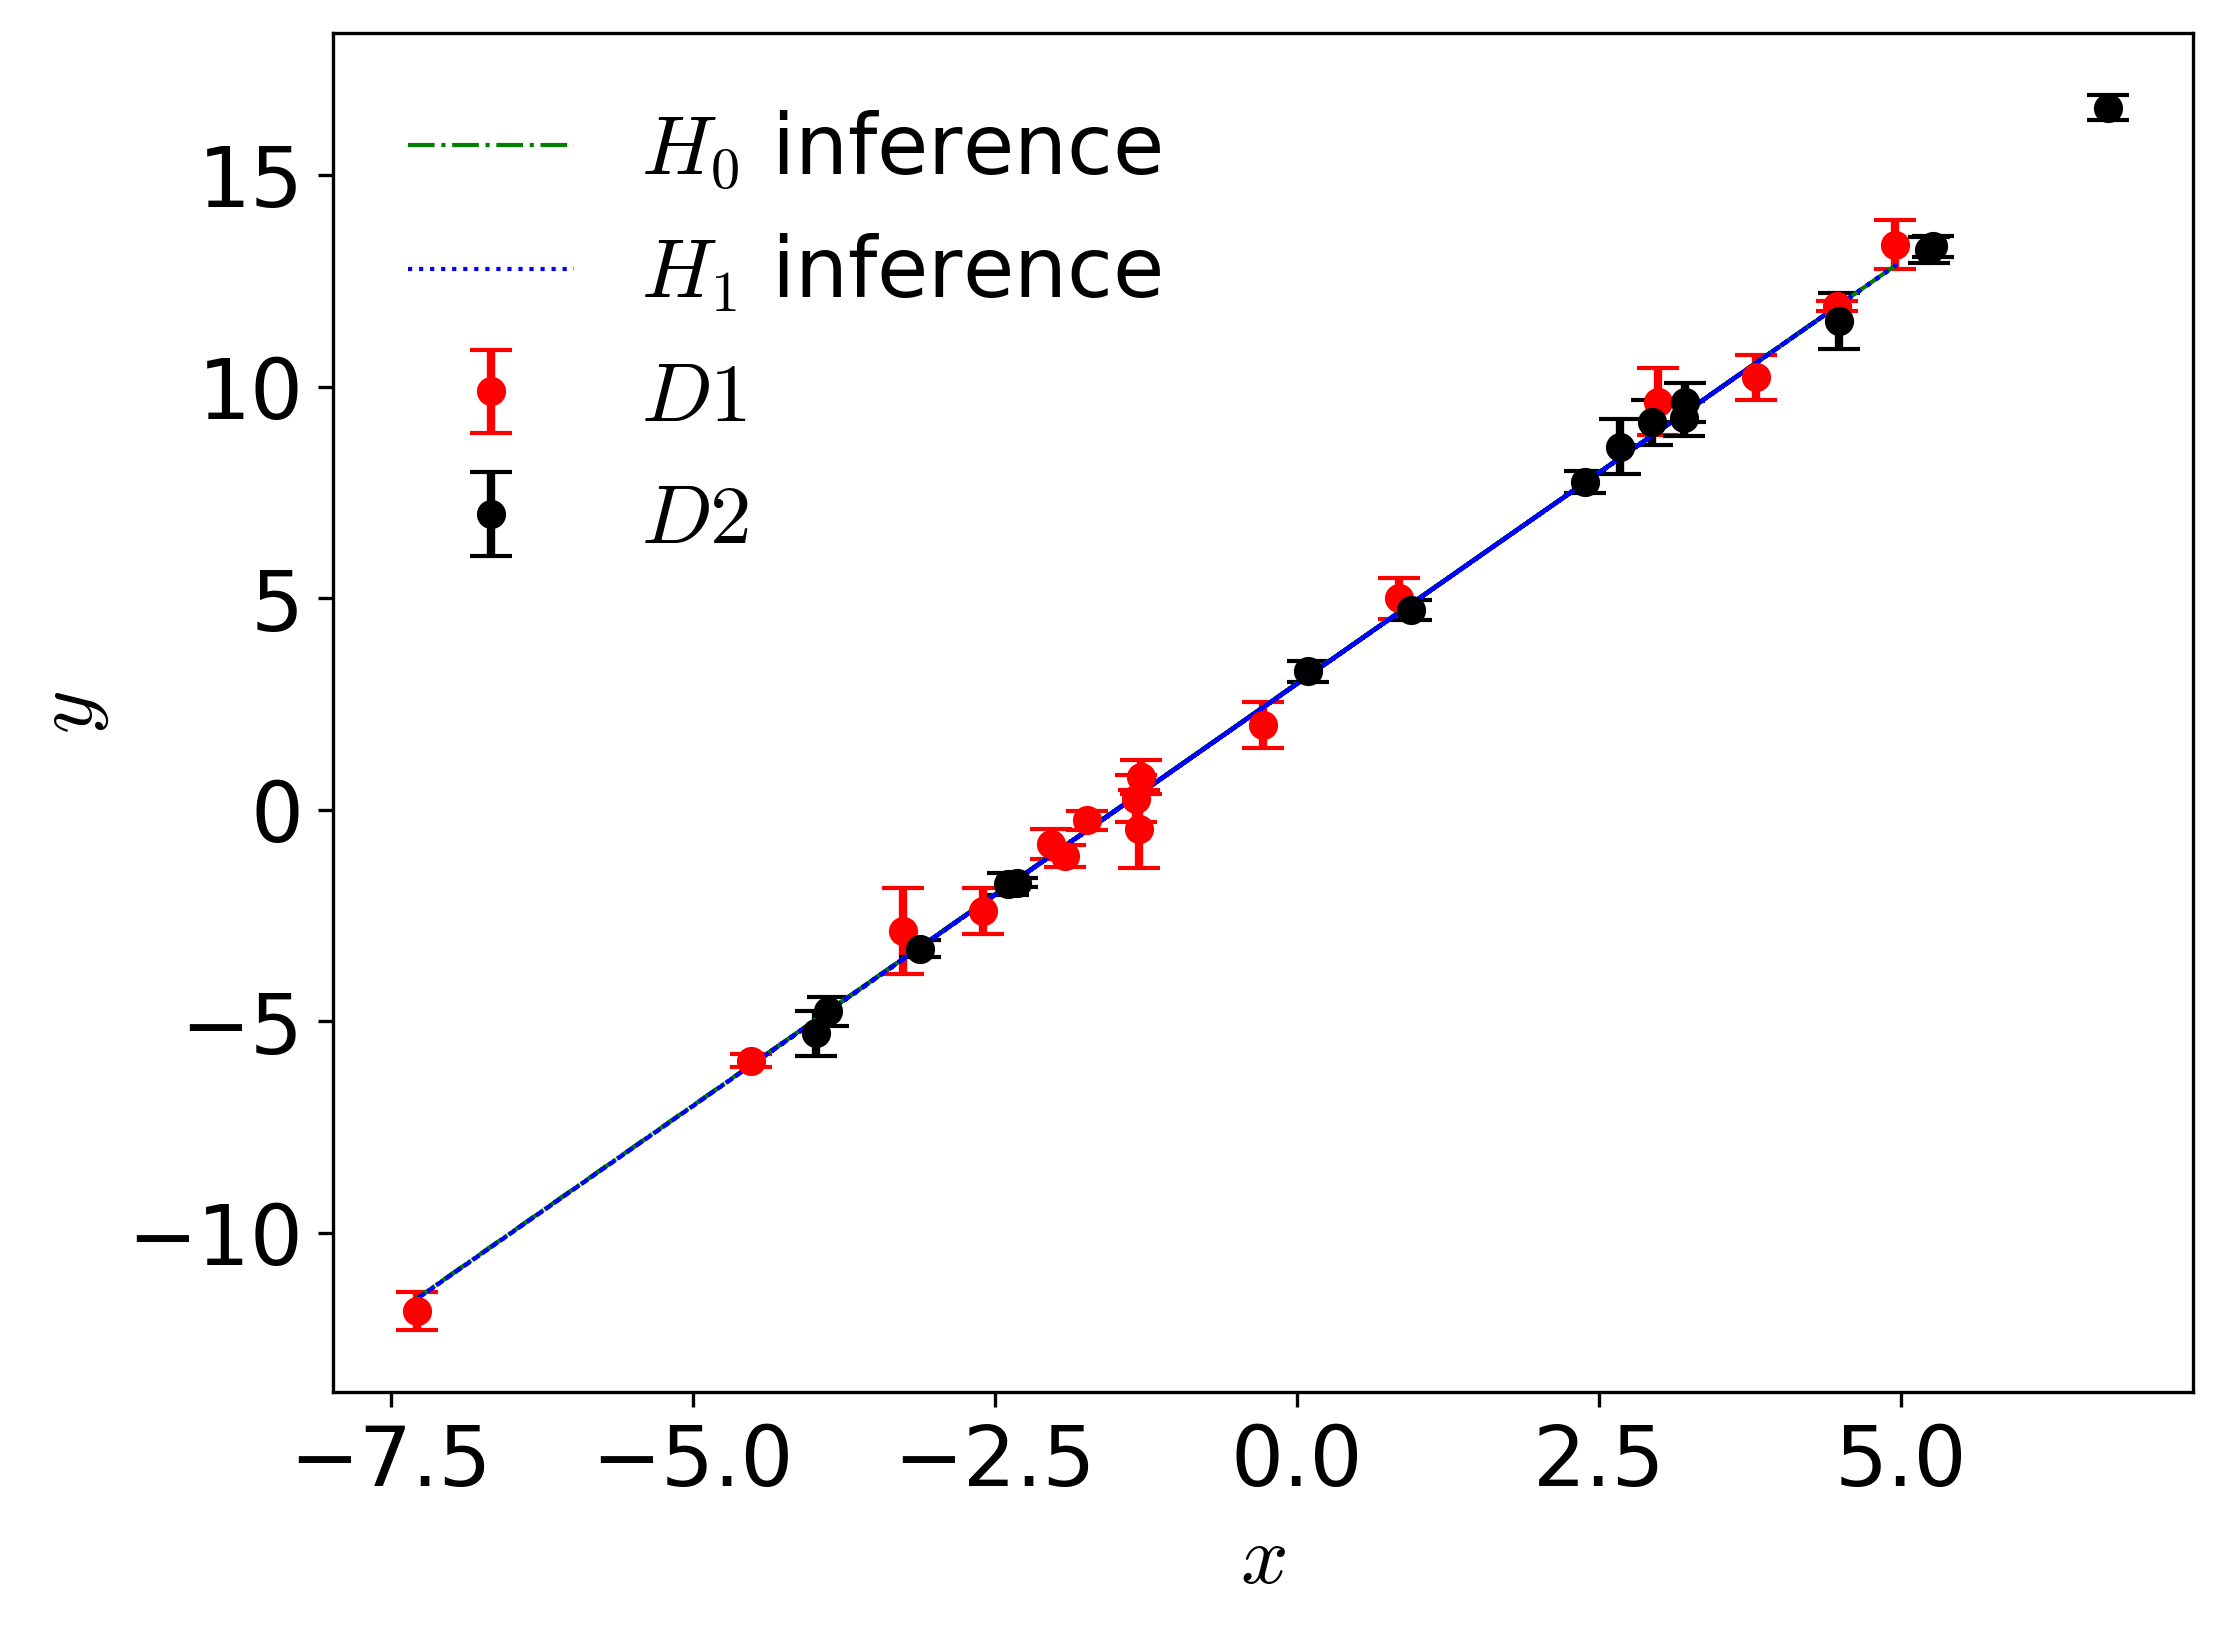
\includegraphics[height=8cm]{stright1.png}
\captionof{figure}{\footnotesize{Our stright-lines inferred by our procedures confronted with the data.}}
\label{stright1}
\end{minipage}

\subsubsection{Case 2}

Now we consider that we have a new set of data and the same theory for the stright-line but suppose that our measurements were kind of distinct. Suppose that we measure the data given in  figure \ref{data_2}. This data corresponds with considering our dataset $D_1$ and changing $D_2$ by 16 new points generated around the line $y=3.5+1.5x$ and with a Gaussian noise with a standard deviation $\sigma = 0.5$. So, our datasets are not auto-consistent between them. Let us make again a parameter estimation for our parameters and look for the differences for bout procedures.

\begin{minipage}{\textwidth}
\centering
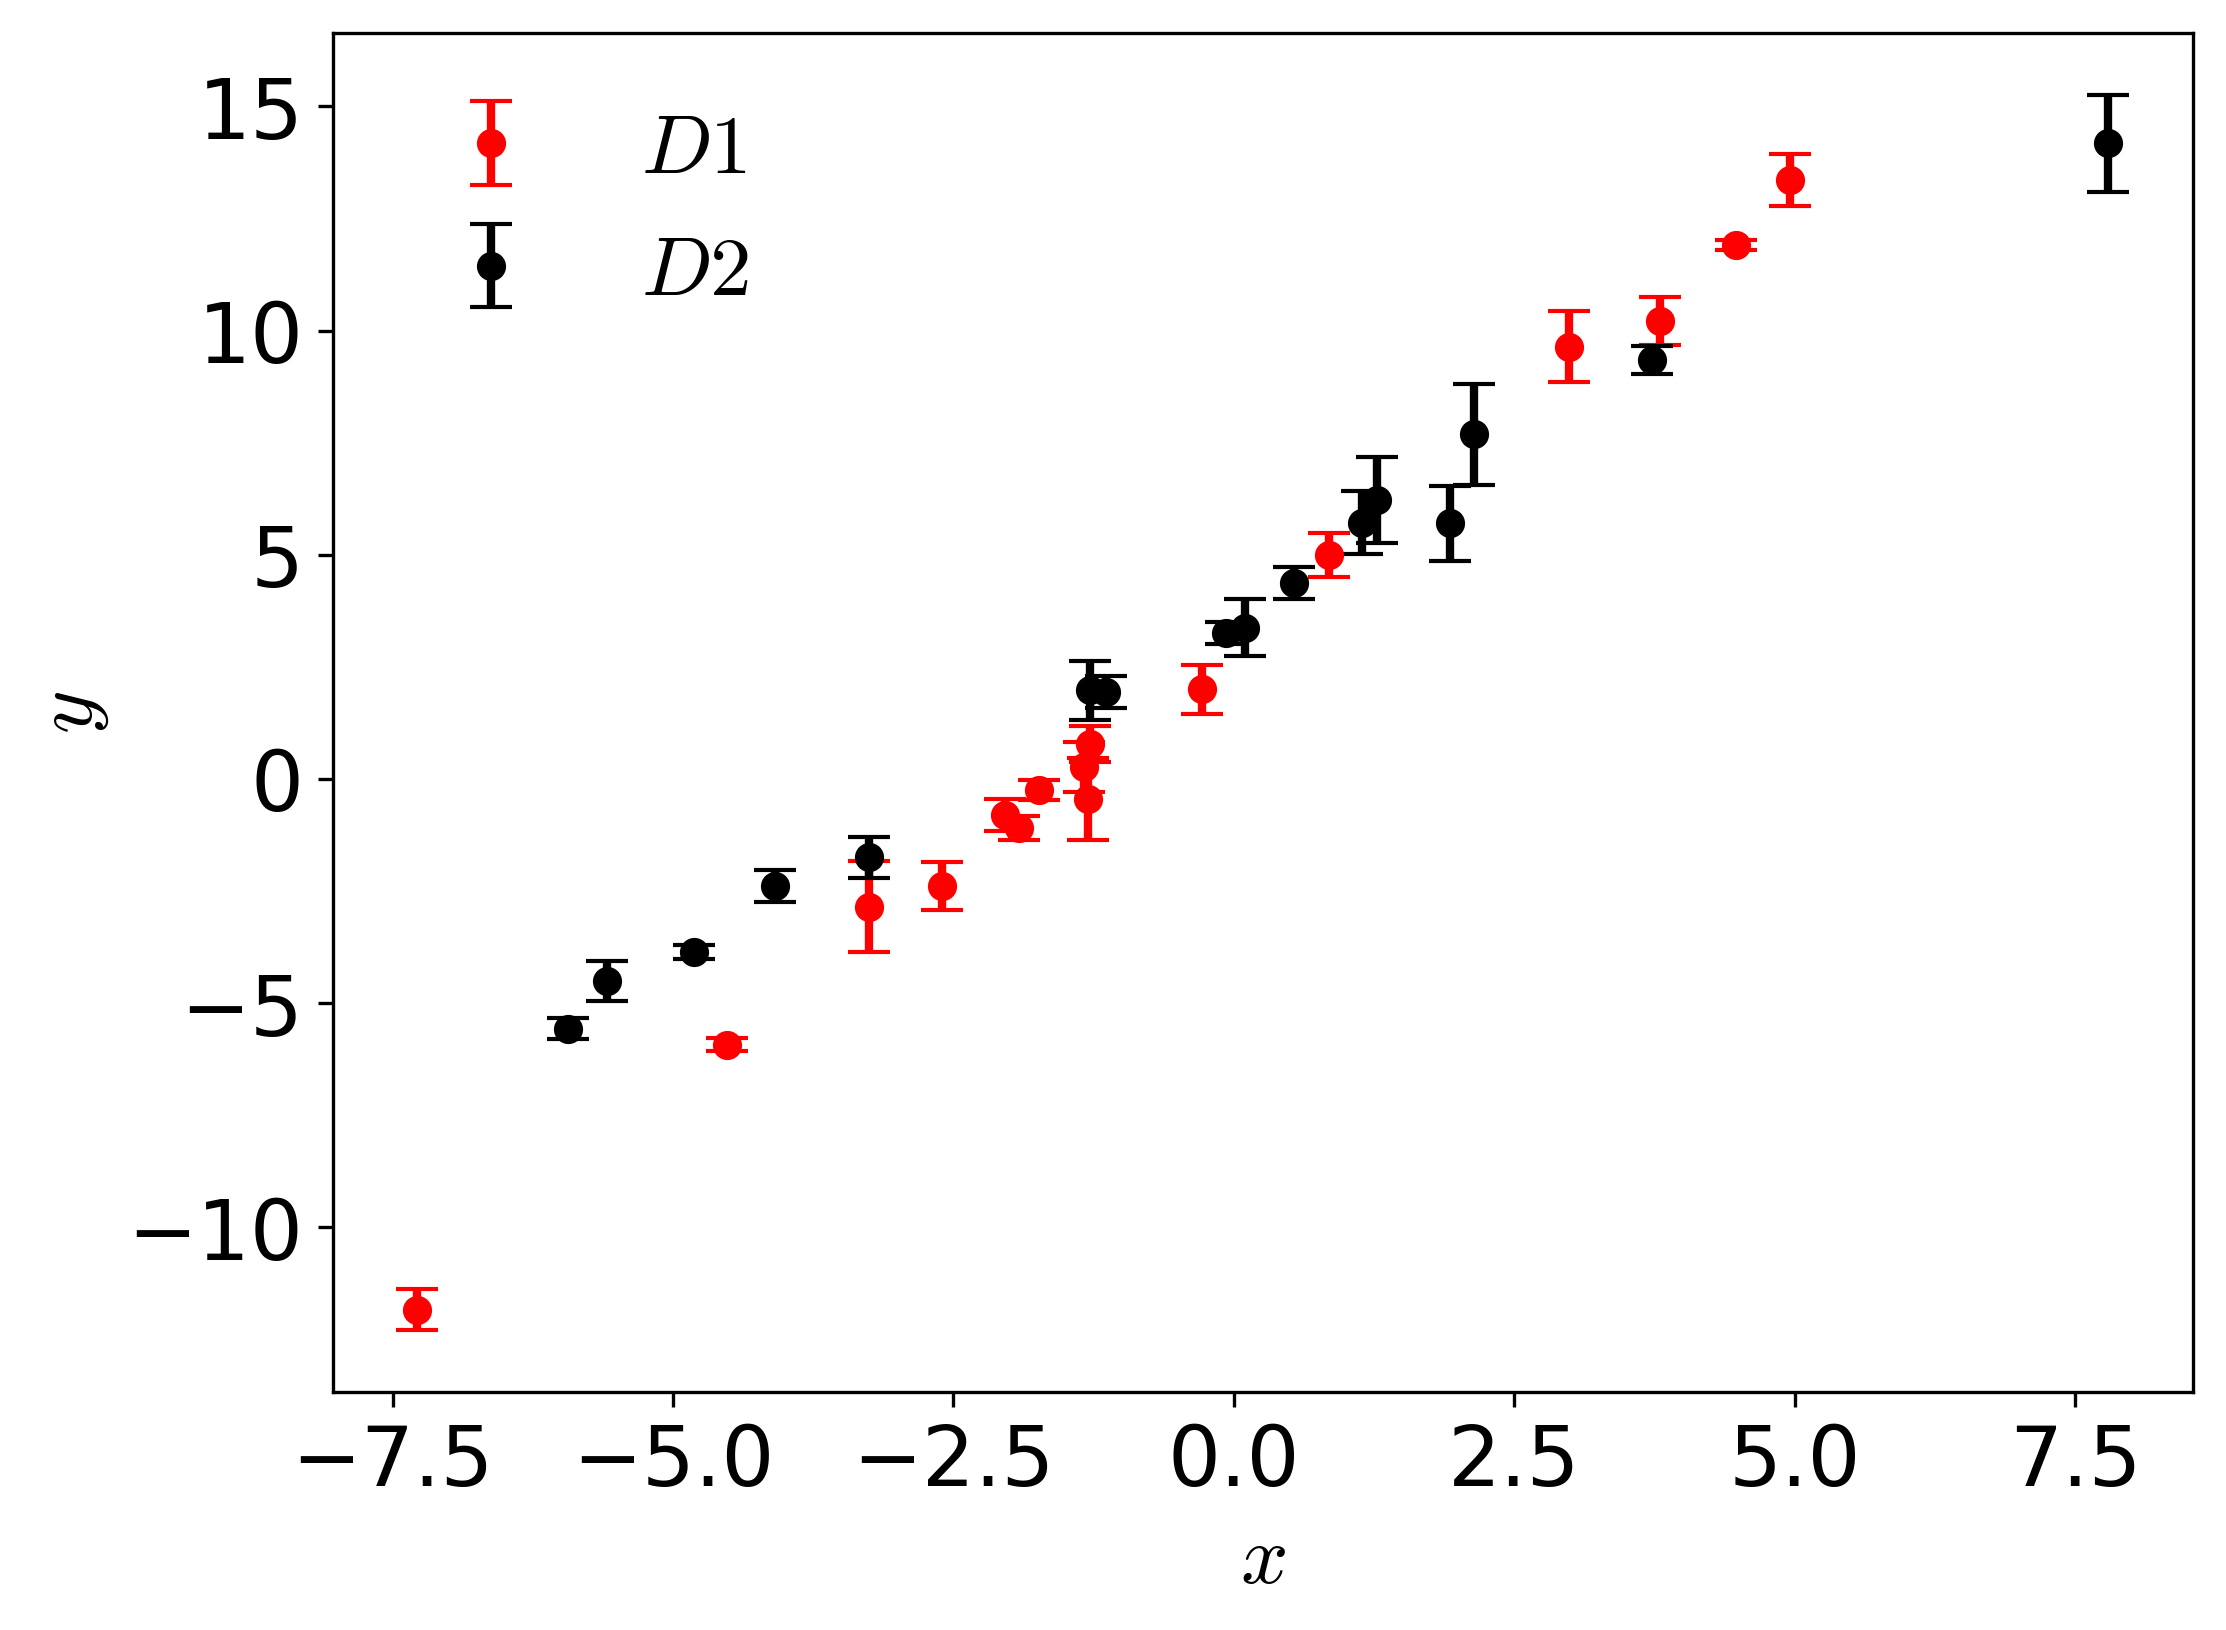
\includegraphics[height=8cm]{data_2.png}
\captionof{figure}{\footnotesize{Datasets $D_1$ and $D_2$ meassured by our stright-line theory.}}
\label{data_2}
\end{minipage}\\ $ $

\textit{Case without hyperparameters. Model $H_0$.-} We followed the same procedure than in Case 1. We computed our posterior and verified that our results converged with the help of the Gelman-Rubin criterion and the autocorrelation plots. Our results can be seen in table \ref{tab2}. Then we plotted our $1-4 \sigma$ confidence regions in figure \ref{contour_3}. What we can see quickly is that our estimation differs so much of the real parameters in our datasets. Of course this is because we are trying to fit a model with non auto-consistent datasets and then we arrive to incorrect results. Now, let us see what happen in the hyperparameters procedure.    

\begin{table}[h!]
\centering
\begin{tabular}{||l|l|l|l||} 
 \hline
 & \textbf{Promedio} & \textbf{Desv. Est.} & \textbf{Gelman-Rubin} \\ [0.5ex] 
 \hline\hline
$a$ & 3.528359 	 & 0.056511 & 1.000153 \\
\hline
$b$ & 1.795464 & 0.014116 	 	 & 1.000393\\ [1ex] 
 \hline
\end{tabular}
\caption{\footnotesize{Our means obtained in our Bayesian estimation for model $H_0$. We also calculated the Gelman-Rubin criterion for each parameter.}}
\label{tab2}
\end{table}

\begin{minipage}{\textwidth}
\centering
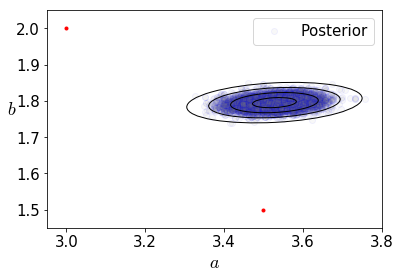
\includegraphics[height=8cm]{contour_3.png}
\captionof{figure}{\footnotesize{Confidence regions for our parameters for model $H_0$.}}
\label{contour_3}
\end{minipage}\\ $ $

\textit{Case with hyperparameters. Model $H_1$.-} We can see in table \ref{tab3} the results of our estimation. In the other side in figure \ref{contour_4} we plotted our posterior. What we can see immediately is that bout approximations are very different for our posterior. While for model $H_0$ we obtained a single region far away of the real values of our data, for model $H_1$ we obtained two locally maximum regions near to our real values for our datasets.  

\begin{table}[h!]
\centering
\begin{tabular}{||l|l|l|l||} 
 \hline
 & \textbf{Promedio} & \textbf{Desv. Est.} & \textbf{Gelman-Rubin} \\ [0.5ex] 
 \hline\hline
$a$ & 3.528359 	 & 0.056511 & 1.000153 \\
\hline
$b$ & 1.795464 & 0.014116 	 	 & 1.000393\\ [1ex] 
 \hline
\end{tabular}
\caption{\footnotesize{Our means obtained in our Bayesian estimation for model $H_1$. We also calculated the Gelman-Rubin criterion for each parameter.}}
\label{tab3}
\end{table}

\begin{minipage}{\textwidth}
\centering
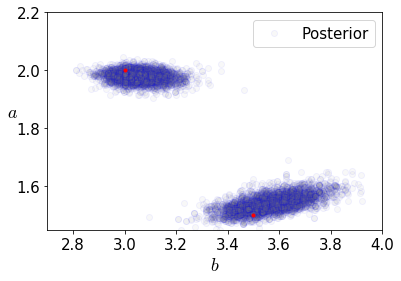
\includegraphics[height=8cm]{contour_4.png}
\captionof{figure}{\footnotesize{Confidence regions for our parameters for model $H_1$.}}
\label{contour_4}
\end{minipage}\\ $ $

Finally we only need to say which method is better. Given the fact that we know \textit{a priori} the real values of our parameters for this example, we could immediately say that the method with hyperparameters is a better approximation than the case without it. However we confirm this assumption by calculating the ratio $K$ between bout models. We obtained
\begin{equation}
K = 37
\end{equation}
which implies that we have a very strong evidence that $H_1$ is better that $H_0$.

\section{Bayesian statistic and Cosmology}

Along the new age of cosmology, observational experiments have been very helpful to confront, eliminate or refined several cosmological models. On this period it has been necessary to improve sensitivity to the experiments in order to achieve stronger constraints on the different models and model's parameters. For example, on CMB satellite experiments, there was a factor of 10 better in sensitive from \textit{COBE} to $WMAP$ and from $WMAP$ to Planck \cite{cmbex}.  On redshift surveys experiments which are interested to map the universe in redshift space, we can compare the 18,000 redshift bright galaxies that were measured by the CfA2 Redshift Survey on 1995 with the \textcolor{red}{[number]} of galaxies that the Sloan Digital Sky Survey (SDSS) measured on \textcolor{red}{(year)} \cite{observ}. In addition there are several new cosmological observations that pretend to update and make our data more precise and that we will need to confront with our models or model's parameters. Such experiments are, for example \textcolor{red}{(Nuevos experimentos. Explicarlos un poco. Aqu\'i entonces comenzar a hablar de que estos nuevos datos se pueden utilizar para constre\~nir par\'ametros).}

\subsection{A first example in parameter inference for Cosmology}

The simplest way to understand how all these concepts can be useful in cosmology is applying them to an example. We consider the typical example in cosmology for parameter inference, which is, we estimate the value of the Hubble parameter $H_0$ at our present time and the density of matter in the Universe $\Omega_m$, considering a $\Lambda CDM$ cosmology. In this section we present the results of a complete work session. We wrote our own Python code using the PyMC Python's module [ref]. For interested readers, the code can be seen in appendix [B]. Notice that this can be used not only in cosmology but also in whatever model that you most prefer; what you need to do in order to prove a new model is only specify it in "pm.model()". 

\subsubsection{What is the model and the theory?}

The standard $\Lambda CDM$ cosmology considers a flat Universe which contains around $\sim 31\%$ of ordinary matter plus dark matter and $\sim 68\%$ of dark energy. In this $\Lambda CDM$ model it is consider that the matter component of the universe follows an equation of state given by $p=0$, while the dark energy is a cosmological constant, i.e. $p=-\rho$. Considering this components, the Universe's dynamics would be given by the Friedmann equation
\begin{equation}
H^2\equiv\left(\frac{\dot a}{a}\right)=H_0^2[\Omega_m(1+z)^3+\Omega_{\Lambda}]
\end{equation}
and the acceleration equation\footnote{We do not show this equation because it is not necessary for our estimation and we do not want to confuse the reader.}. Here $H$ is the Hubble parameter, $H_0$ corresponds with the Hubble parameter at present, $\Omega_m$ and $\Omega_\Lambda$ is the matter and dark energy densities at our epoch and follows the constraining condition $\Omega_m+\Omega_\Lambda=1$, and $z$ is the redshift which is associated with a time parameter; $z=0$ is at present. Notice that thanks to the constraining condition we can rewrite $\Omega_\Lambda=1-\Omega_m$ and then we can reduce by one the number of parameters in the model. 
\subsubsection{The observables and the data}

It is possible to measure $H(z)$ by using what it is known as the \textit{cosmic chronometer} approach \cite{Hz}. We use the data reported in \cite{Hzdata} as our data for our estimation. A plot of them can be seen in figure \ref{HzData}.

\begin{minipage}{\textwidth}
\centering
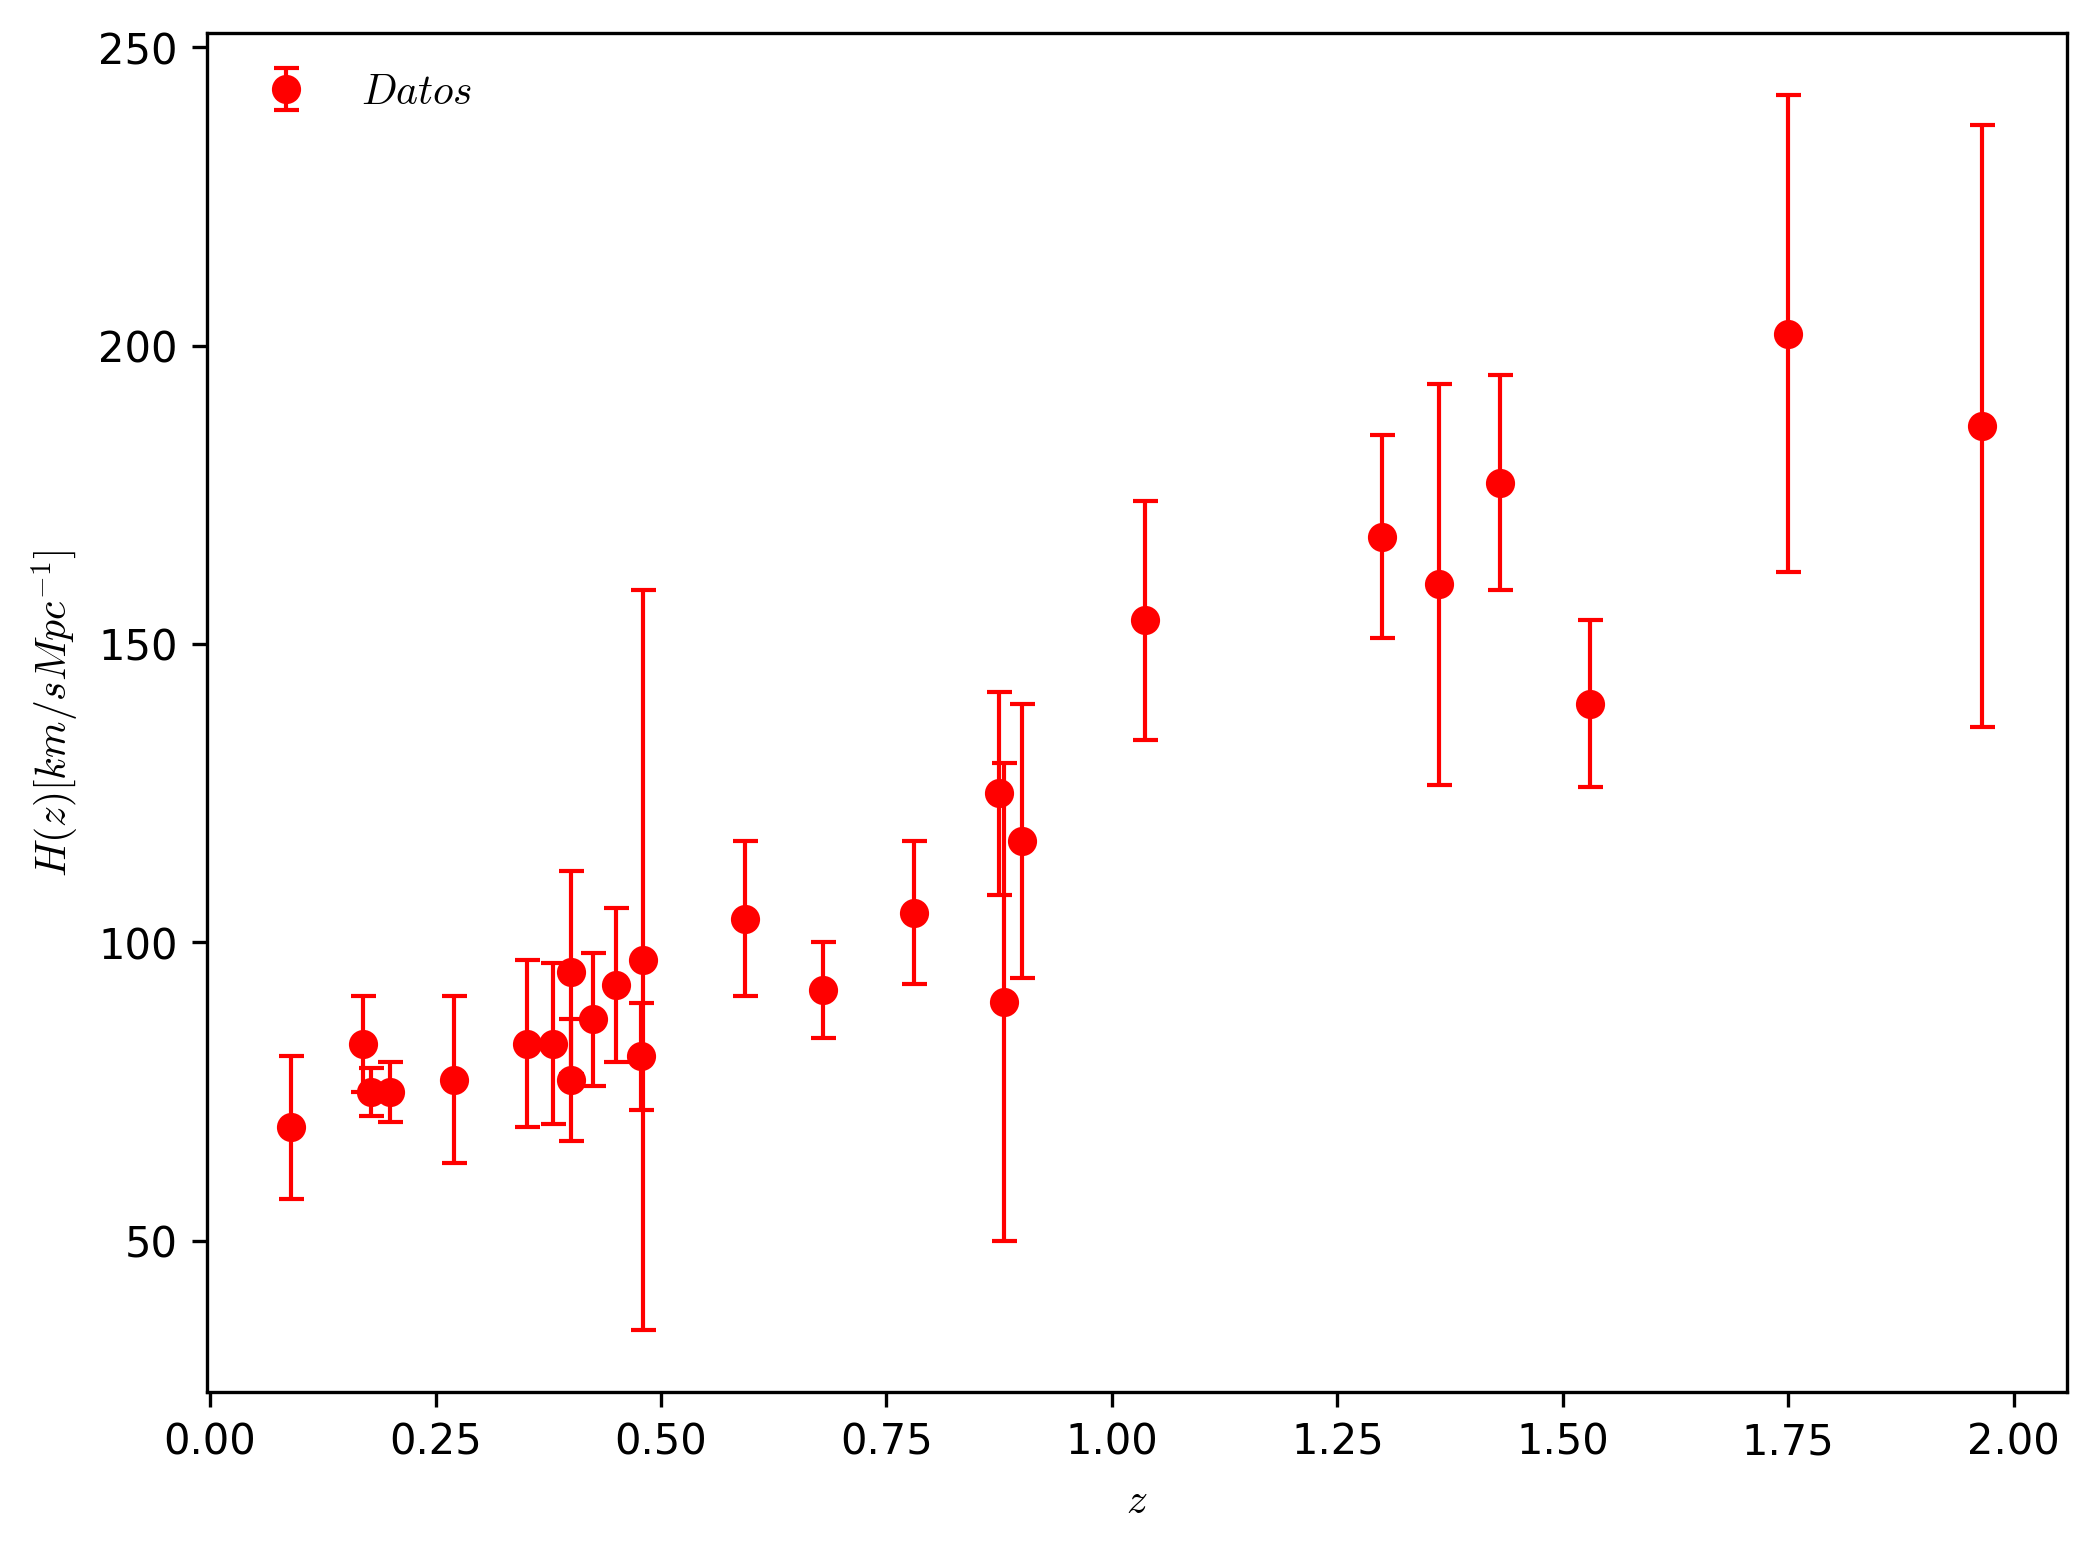
\includegraphics[height=8cm]{Hzdata.png}
\captionof{figure}{\footnotesize{Multiple MCMC. We calculate 5 Markov chains to estimate convergence of our chains.}}
\label{HzData}
\end{minipage}

\subsubsection{Inferring the free parameters of the model}

Now, giving a model and a set of data, we are ready to apply what we have learned until now. First of all, notice that the only free parameters in our model are $\Omega_m$ (or $\Omega_\Lambda$) and $H_0$. We suppose that we don't know anything about our free parameters, in such case a good prior for them is a Uniform distribution. However, in order to simplify our life we consider that we know something about the limit values for both parameters,  say: $\Omega_m\in [0.1,1]$ and $H_0\in [10,100]$. In this way we have as our priors
\begin{subequations}
\begin{equation}
\Omega_m\sim U[0.1,1]
\end{equation}
\begin{equation}
H_0\sim U[10,100]
\end{equation}
\end{subequations} 
\subsection{What is next?}

\textcolor{red}{Una vez de que ya entedimos los procedimientos para la inferencia de par\'ametros, hablar de que el siguiente paso es saber que hay varios c\'odigos que ya hacen todo lo que vimos (tanto la cosmolog\'ia, como la estad\'istica) y que es mejor aprender a moverles que andar haciendo nuestro propio código (quiz\'as)}
%\subsubsection{Cosmological codes}

%Now a days there are a lot of cosmological Boltzmann codes that are free on the web and can help us to prove our cosmological models. The most popular of them are: CMBFAST \cite{cmbfast1}, CMBEASY \cite{cmbeasy}, CAMB \cite{camb1} (some useful references for CAMB: \cite{camb2,camb3,camb4}) and CLASS \cite{class1} (a useful reference for CLASS: \cite{mont1}). All of them are used for calculating the linear CMB anisotropy spectra based on integration over the sources along the photon past light cone.

%\subsubsection{CMBFAST}

%As can be seen in the NASA web-page \cite{cmbfast1}, CMBFAST is a code, written by U. Seljak and M. Zaldarriaga, for calculating the linear cosmic microwave background (CMB) anisotropy spectra based on integration over the sources along the photon past light cone. In this approach the temperature anisotropy is written as a time integral over the product of a geometrical term and a source term. The code can be downloaded as an interface in \cite{cmbfast1} where the user introduce entry parameters required by CMBFAST and when it is run, some of the results are displayed graphically; all of the results are stored in files and made available for the user.

%\subsubsection{CAMB}

%CAMB is a code for anisotropies in the Microwave Background. It was written by Antony Lewis and Anthony Challinor in the f90 language and based on CMBFAST. It can be downloaded in \cite{camb1}. Some useful references for the use of this code can be found in \cite{camb2}, \cite{camb3} and \cite{camb4}.

%\subsubsection{CLASS}

%As can be seen in the wave-page of CLASS \cite{class1}, the purpose of CLASS is to simulate the evolution of linear perturbations in the universe and to compute CMB and large scale structure observables. Its name also comes from the fact that it is written in object-oriented style mimicking the notion of class. The code was written in the C language. It can be downloaded in \cite{class1} and some useful references for the use of the code can be found in \cite{mont1}.

\subsubsection{Statistical codes}

Once our cosmological model is established we need a statistical code which can help us to estimate the free parameters of our model. A first idea could be continuing programing our own MCMC code, but, as it is expected, while the number of free parameters of our model increases, it is more challenging to construct an efficient code. Fortunately there are several MCMC codes free to download on-line that can make this homework taking as our theory the cosmological codes showed above. In this section we review the most common of them.

\textit{Monte Python}.-
Monte Python is a Monte Carlo code for Cosmological Parameter extraction  that can be downloaded in \cite{MP1}. It contains likelihood codes of most recent experiments, and interfaces with the Boltzmann code Class for computing the cosmological observables.

The code contains several sampling methods available: Metropolis-Hastings, Nested Sampling (through MultiNest), EMCEE (through CosmoHammer) and Importance Sampling. If you are interested to work with this parameter inference code you can get help in \cite{mont1} and \cite{MP2}.

\textit{CosmoMC}.- CosmoMC (to download \cite{cosmomc}) is a fortran 2003 MCMC engine for exploring cosmological parameter space. It contains Monte Carlo samples and inportance sampling. It containg likelihoods of most recent experiments, and interfaces with CAMB.

\textit{SimpleMC}.- SimpleMC is a MCMC code for cosmological parameter estimation where only expansion history matters. It was written by Anže Slosar and Jose Vazquez and can be downloaded on \cite{simplemc}

\subsection{Some examples}
\textcolor{red}{Examples of cosmology}
\subsection{Conclusions}
\appendix
\section{A. A simple MCMC python code}

Here we show our MCMC written in Python. This code is very simple and its propose is to help the reader to understand how to programing a MCMC code. However, if you are interested in more sophisticated algorithms you can see the PyMC module of python [ref]. We wrote our code using the jupyter notebook [ref] which is a excelent editor when we have a program no much extense.  

\begin{figure}[h!]
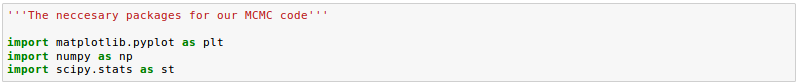
\includegraphics[height=2cm]{c1.png}
\end{figure}
\begin{figure}[h!]
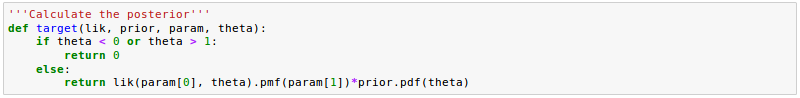
\includegraphics[height=2.339cm]{c2.png}
\end{figure}
\begin{figure}[h!]
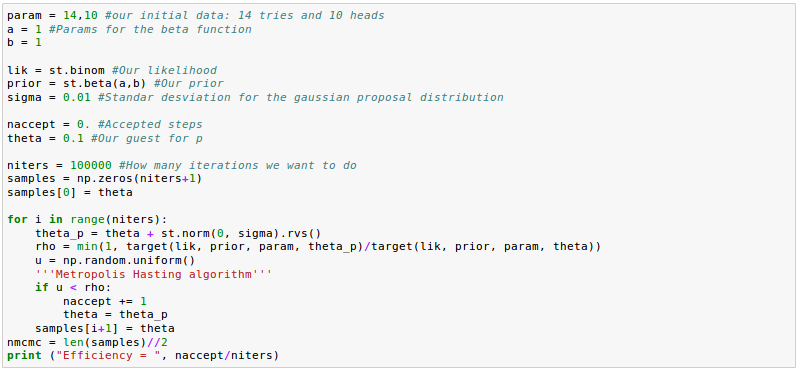
\includegraphics[height=8.85cm]{c3.png}
\end{figure}
\begin{figure}[h!]
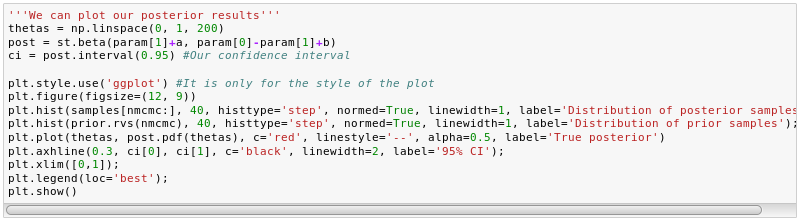
\includegraphics[height=5.21cm]{c4.png}
\end{figure}

\begin{thebibliography}{9}
\bibitem{debate} The Shapley - Curtis Debate in 1920, $https://apod.nasa.gov/diamond_jubilee/debate_1920.html$, visited on December 2017
\bibitem{bayeslecture}B.J.K. Kleijin; Bayesian statistic, lecture notes 2015
\bibitem{AlanH} Alan Heavens; Statistical techniques in cosmology; May 2010
\bibitem{RobT} Roberto Trotta; Bayes in the sky: Beyesian inference and model selection in cosmology; March, 2008
\bibitem{LiV} Licia Verde; Statistical methods in cosmology; Nov, 2009
\bibitem{RobTr}Roberto Trotta; Bayes Methods in Cosmology; Jan, 2017
\bibitem{Fisher}Fisher R.A. (1935) \textit{J. Roy. Stat. Soc.} \textbf{98}, 39
\bibitem{NR}Numerical Recipes
\bibitem{mcmc1}anner, M. (1993)
Tools for Statistical Inference, Method for
Exploration of Posterior Distributions and Likelihood Func-
tions.
\bibitem{mcmc2}Gilks, W., Richardson, S. and Spiegelhalter, D. (1996)
Markov Chain
Monte Carlo in Practice.
\bibitem{mcmc3}Gelman, A., Carlin, J., Stern, H and Rubin, D. (1995)
Bayesian Data
Analysis.
\bibitem{mcmc4}oss, Sheldon, (1989)
Introduction to Probability models 4th
Edit.
\bibitem{metr} Metropolis, N., Rosenbluth, A.W., Rosenbluth, M.N., Teller, A.H., Teller, E.: Equation of state
calculations by fast computing machines. J. Chem. Phys.
21
, 1087–1092 (1953)
\bibitem{LicV2} Verde L., astroph/0712.3028 (2007)-
\textit{http://www.behind-the-enemy-lines.com/2008/01/are-you-bayesian-or-frequentist-or.html}
\bibitem{observ}218.163.109.230 et al. (2004–2014); \textit{Observational cosmology -
30h course}.
\bibitem{gibbs1} A. Smith and G. Roberts, J. R. Statist. Soc. B
55
3–23 (1993).
\bibitem{gibbs2} Ilker Yildirim, Bayesian Inference: Gibbs Sampling, August 2012
\bibitem{hamiltonian1}K. M. Hanson, Markov Chain Monte Carlo posterior sampling with the Hamiltonian method, in M. Sonka and K. M. Hanson eds, Medical Imaging: Image Processing
Vol. 4322, Proc. SPIE, pp. 456–467.
\bibitem{Hamiltonian2} Radford M. Neal, MCMC using Hamiltonian dynamics, arXiv:1206.1901v1 [stat.CO]
\bibitem{importance} Surya T. Tokdar and Robert E. Kass, Importance Sampling: A review, DOI: 10.1002/wics.56
%
%
%
%
\bibitem{cmbex} K. N. Abazajian, K. Arnold, J. Austermann, B. A. Ben-
son, C. Bischoff, J. Bock, J. R. Bond, J. Borrill, E. Cal-
abrese,  J.  E.  Carlstrom,  et  al.,  ArXiv  e-prints  (2013),
1309.5383.
\bibitem{cmbfast1}$https://lambda.gsfc.nasa.gov/toolbox/tb_cmbfast_ov.cfm$
\bibitem{cmbeasy}$http://adsabs.harvard.edu/abs/2010ascl.soft07004D$
\bibitem{camb1}$http://camb.info/$
\bibitem{camb2}$http://camb.info/readme.html$
\bibitem{camb3}$http://cosmocoffee.info/viewforum.php?f=11$
\bibitem{camb4} $http://cosmologist.info/notes/CAMB.pdf$
\bibitem{class1} http://class-code.net/
\bibitem{mont1}Zumalacarregui Miguel; \textit{CLASS, hi class and Monte Python basics IFT School on Cosmology Tools}; March 11, 17.
\bibitem{MP1}\textit{http://baudren.github.io/montepython.html}
\bibitem{MP2}Benjamin Audren, \textit{Monte Python documentation, Release 2.2.0}; October 21, 2015
\bibitem{cosmomc}$http://cosmologist.info/cosmomc/$	
\bibitem{simplemc}$https://github.com/ja-vazquez/SimpleMC$
%
%
%
%
%
%
\bibitem{Hz}R. Jimenez and A. Loeb, “Constraining Cosmological Parameters Based on Relative Galaxy Ages,”
ApJ, vol. 573, pp. 37–42, July 2002.
\bibitem{Hzdata}Michele Moresco, Raul Jimenez, Licia Verdec, Andrea Cimatti, Lucia Pozzetti, Claudia Maraston, \textit{Constraining the time evolution of dark energy, curvature and neutrino properties with cosmic chronometers}, Journal of Cosmology and Astroparticle Physics, (2016), arXiv:1604.00183v1 [astro-ph.CO]
\bibitem{autocor} Model checking diagnostic, PyMC 2.3.6 documentation, link: \textit{https://pymc-devs.github.io/pymc/modelchecking.html}
\bibitem{thin}William A. Link and Mitchell J. Eaton, On thinning of chains in MCMC, Methods in ecology and evolution,
\bibitem{mcmcmc}W. D. Vousden, W. M. Farr and I. Mandel,\textit{Dynamic temperature selection for parallel-tempering in Markov chain Monte Karlo simulations}, MNRAS (January 11, 2016) Vol. 455 1919-1937, arXiv:1501.05823 [astro-ph.IM]
\bibitem{hiperp}Lahav O., Bridle S. L., Hobson M. P., Lasenby A. N., $\&$ Sodre L., 2000, MN-RAS, 315, 45
\bibitem{hiperp1}Hobson M. P., Bridle S. L., $\&$ Lahav O., 2002, MNRAS, 335, 377 (HBL
\bibitem{hiperp2}e
ff
reys H.,
The Theory of Probability
, Oxford University Press, 1961.
\bibitem{importancesampling}Surya T Tokdar and Robert E Kass, Importance sampling: A Review, DOI: 10.1002/wics.56

\end{thebibliography}
\end{document}

